\documentclass[russian, utf8, 12pt]{eskdtext}
\newcommand*{\No}{\textnumero}
\ESKDdepartment{Кафедра Систем Управления и Информатики}
\ESKDcompany{Университет ИТМО}
\ESKDdocName{Устройство для измерения плотности жидкости}
\ESKDsignature{КСУИ.124.P3340.001 ПЗ}
\ESKDauthor{Овчаров А.О.}
\ESKDchecker{Быстров С.В.}
\ESKDnormContr{Быстров С.В.}
\ESKDcolumnIX{\small Университет ИТМО\\
Кафедра СУиИ}

\usepackage[hidelinks]{hyperref}
\usepackage{pscyr}

\usepackage{tocloft}
\renewcommand{\cftaftertoctitle}{\hfill}
\renewcommand{\cfttoctitlefont}{\hspace{7cm}\Large\bfseries}	%KOSTIL'
\renewcommand{\cftaftertoctitle}{\hfill}
\renewcommand{\cftdot}{.}
\renewcommand{\cftsecleader}{\cftdotfill{\cftdotsep}} % for sections
\makeatletter

\usepackage{wrapfig}
\usepackage{graphicx}
\graphicspath{{images/}}
\DeclareGraphicsExtensions{.pdf, .jpg, .png}

\usepackage{caption}
\captionsetup[table]{singlelinecheck=false} % Заголовок таблиц слева
\captionsetup[table]{aboveskip=2pt,belowskip=2pt} %belowskip=6pt
% Позиционирование заголовка

\usepackage{tikz}
\usepackage{array}

\usepackage{geometry} %способ ручной установки полей
\geometry{top=2.5cm} %поле сверху
\geometry{bottom=2.5cm} %поле снизу
\geometry{left=2.5cm} %поле справа
\geometry{right=1cm} %поле слева


%%%%%%%%%%%%%%%%%%%%%%%%%%%%%%%%%%%%%%%%%%%%%%%%%%%%5
\usepackage[texcoord]{eso-pic}

\newcommand\PlaceText[3]{%
\begin{tikzpicture}[remember picture,overlay]
\node[outer sep=0pt,inner sep=0pt,anchor=south west] 
  at ([xshift=#1,yshift=-#2]current page.north west) {#3};
  \draw[line width = 1pt] (9,-0.5) -- (9,-1.9) -- (2,-1.9);
\end{tikzpicture}%
}



%%%%%%%%%%%%%%%%%%%%%%%%%%%%%%%%%%%%%%%%%%%%%%%%%%%%%%%%
% Структурный элемент и его стиль
\newcommand*{\StructSection}[1]{\centerline{\Large \bfseries #1}\vspace{21pt}}
% Отступы от заголовка по ЕСКД
\ESKDsectSkip{section}{21pt}{21pt}
\ESKDsectSkip{subsection}{21pt}{21pt}

\usepackage[final]{pdfpages}

\begin{document}
% Title
\ESKDthisStyle{empty}
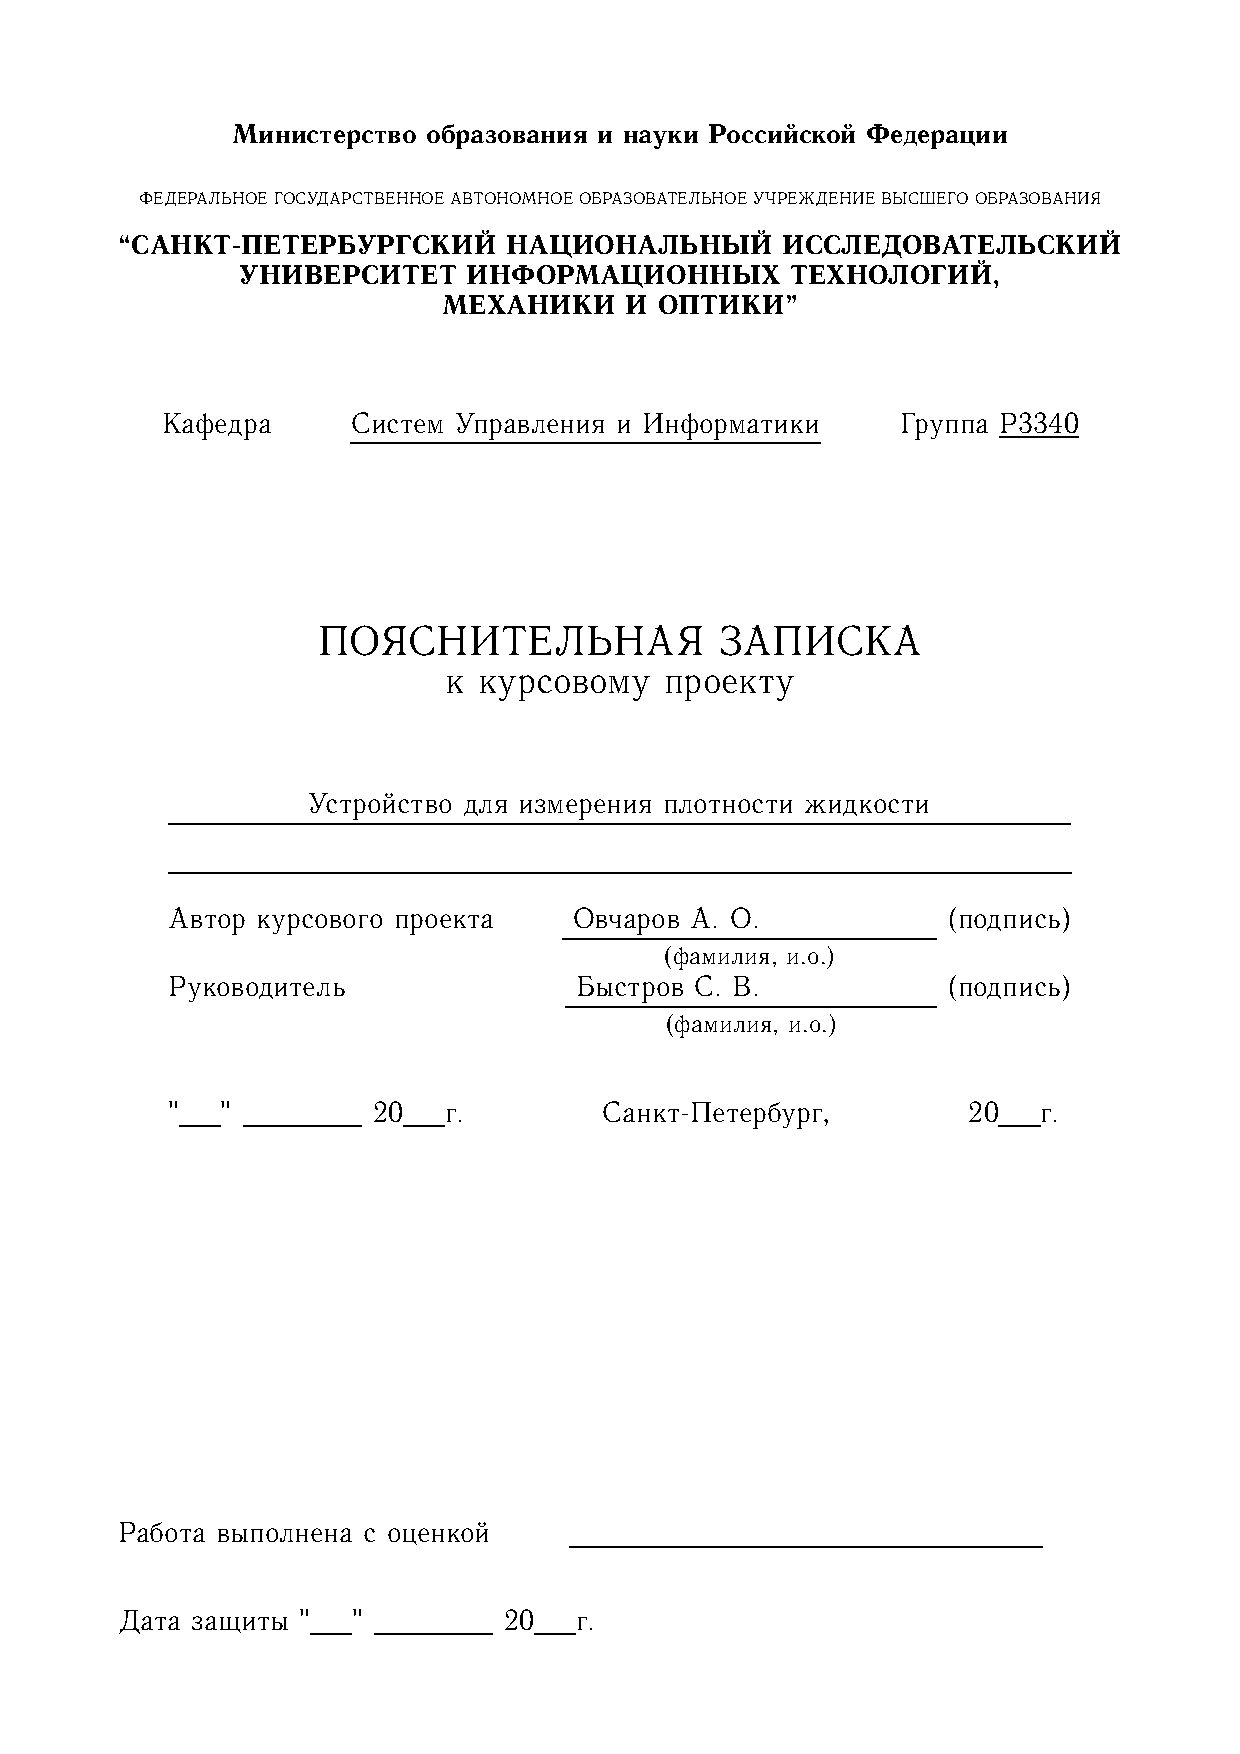
\includepdf {../TitlePage.pdf}
\newpage
\setcounter{page}{4}
\AddToShipoutPictureBG*{%
\PlaceText{76}{40}{\rotatebox{180}{КСУИ.224.P3340.001 ПЗ}}}
\ESKDthisStyle{formII}
\tableofcontents
\thispagestyle{empty}
\newpage

%
% -------------------------------------------------------------------------------
% Введение
{\StructSection{Введение}
\addcontentsline{toc}{section}{Введение}}

Люди могли измерять плотность уже в древности. Так, например, Архимед в своем законе использует плотность жидкости. В настоящее время необходимость измерения плотности жидкости выросла до такой степени, что было выпущено множество статей и книг по способам и приборам измерения плотности. \par
\textbf{Плотностью} $\rho$ однородного вещества называют отношение его массы $m$ к объему $V$.
\begin{equation}
	\rho = \frac{m}{V}
\end{equation}
Для неоднородного вещества плотность определяется как предел отношения массы к объему, когда объем стягивается к точке, в которой определяется плотность:
\begin{equation}
	\rho = \lim_{\Delta V\rightarrow0}{\frac{\Delta m}{\Delta V}}
\end{equation}
где $\Delta m$ - масса элементарного объема $\Delta V$.

Также в ряде отраслей науки и техники для характеристики вещества применяю \textbf{относительную плотность}, представляющая собой отношение плотности рассматриваемого вещества к плотности другого, условного, вещества при определенных физических условиях. В качестве условного вещества обычно принимают дистиллированную воду. \par

Существует достаточно много методов измерения плотности, на которых основана работа большого количества приборов. \par

Большую группу методов называют \textbf{поплавковою-весовыми}, данные методы основаны на определении выталкивающей силы, действующее на испытуемое тело или вспомогательное тело (поплавок). Эта сила в соответствии с законом Архимеда прямо пропорциональная плотности среды, в которую погружено тело. Сюда можно отнести методы ареометра, гидростатического взвешивания, 
, флотационный. \par

Следующую группу образуют \textbf{гидростатические} методы измерения, которые базируются на зависимости статического давления столба жидкости или газа постоянной высоты от их плотности. \par

Выделяют также \textbf{гидродинамические} методы, основанные на зависимости от полосни таких физических величин, как скорость истечения струи жидкости или газа из отверстия, сила удара струи о преграду, скорость падения тела в жидкости, энергия потока вещества, динамическое давление и др. \par

На сегодняшний день развились также и новые методы определения жидкости. \textbf{Радиационный} метод основан на зависимости плотности от ослабления радиоактивного излучения облученного вещества. \textbf{Ультразвуковой} метод основан на скорости распоряжения ультразвуковых волн в веществе. \textbf{Вибрационный} метод основан на зависимости плотности от параметров упругих колебаний, сообщаемых сосуду с исследуемым веществом. \par

Приборы, осуществляющие измерение плотности называются \textbf{плотномерами}. Далее будут рассмотрены плотномеры, работающие по разным принципам.

В работе требуется разработать систему, позволяющую измерять плотность жидкости в соответствии с условиями, описанными в таблице 1.

\begin{table}[h!] 
\renewcommand{\arraystretch}{1.2}
\caption{Данные для проектирования}
\begin{tabular}{|m{0.48\textwidth}|m{0.47\textwidth}|}
	\hline
	Диапазон измерения плотности & от 600 до 1800 кг/м$^3$ \\ \hline
	Температора измерений & 20 $^\circ\text{C}$ \\ \hline
	Допустимая погрешность измерения & 5 \% \\ \hline
	Напряжение питания & 220 В 50 Гц \\ \hline
	Выходной сигнал устройства & 8-ми разрядный параллельный код \\ \hline
	Линия связи для выходного сигнала устройства & RS-485 \\ \hline
\end{tabular}
\end{table}

\newpage
%
% --------------------------------------------------------------------
% Сравнительный анализ существующих решений
\section{Сравнительный анализ существующих решений}

Далее мы сравним четыре различных по методу измерения плотномера. Из них выберем один метод измерения, при котором измерительные прибор будет соответствовать основным критериям. \par

Главным критерием выбора плотномера является малость габаритов измерительного устройства, соответствии заданным данным и малая инерционность измерений. \par

\subsection{Поплавковый плотномер}

Действие поплавковых плотномеров основано на зависимости плотности от перемещения поплавка от нейтрального положения или наоборот, перемещения жидкости при неподвижном поплавке. \par

На рисунке 1 представлена схема плотномера с плавающим поплавком. Жидкость по трубке 6 поступает в переливной сосуд 5, а оттуда по проводящей трубке 4 поступает в измерительный сосуд 2, который также снабжен переливным устройством. Требуемая скорость потока устанавливается диафрагмой 10. Для отвода излишков воды имеется трубка 9. В результате действия выталкивающей силы поплавок перемещается по вертикали, тем самым сердечник совершает те же перемещения вдоль индуктивного датчика 7, включенный в схему измерительного моста 1. Для коррекции показаний изменение температуры, используется датчик температуры 3. \par 

\begin{figure}[h!]
	\centering
	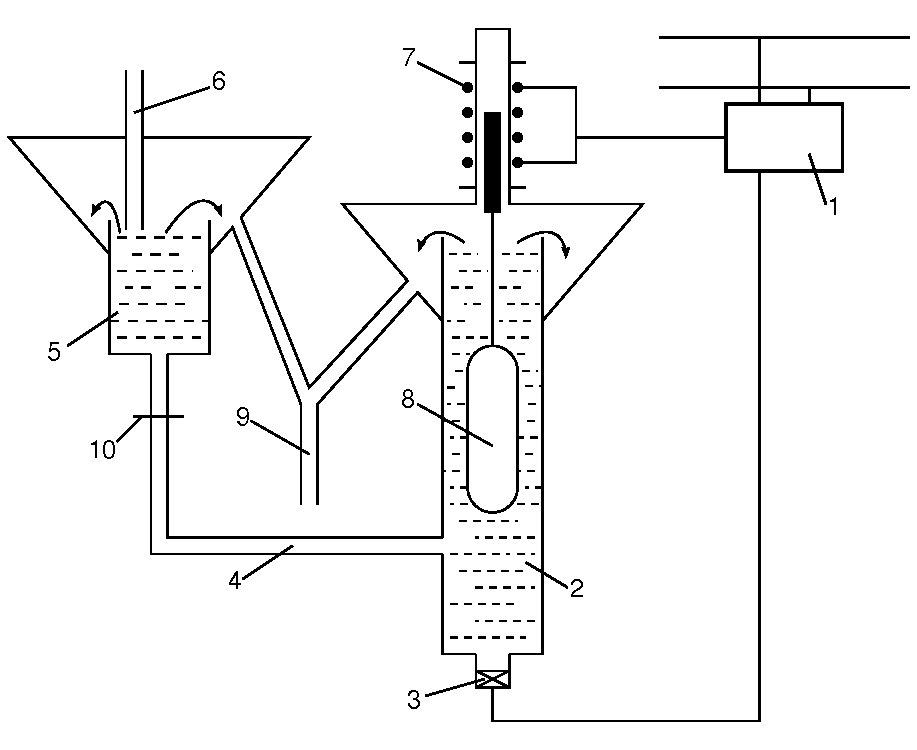
\includegraphics[width = 0.6\textwidth] {FloatDensityMeter.pdf}
	\caption{Схема плотнометра с плавающим поплавком}
\end{figure}

\newpage

На поплавок действует выталкивающая сила по закону Архимеда, эта сила компенсирует вес тела поплавка и вес миниска. В силу малости выталкивающей силы миниска в воздухе, она не учитывается. Таким образом сила Архимеда включает в себя две части:

\begin{align}
	P_a & = (v + lS)\rho g \\
	P_c & = (V - v - lS)D
\end{align}
где выражение (1) характеризует вес жидкости в обхеме погруженной части стержня, а выражение (2) вес воздуха в объеме погруженно части стержня. \par

Тогда можем записать закон Архимеда, с учетом того, что поплавок не тонет: 
\begin{equation}
	m + La\rho = (v + lS)\rho + (V - v - lS)D
\end{equation}
или
\begin{equation}
	m - VD + La\rho = (v + lS)\rho - (v + lS)D
\end{equation}
здесь $v$ - объем нижней части поплавка без стержня; $l$ - длинна погруженною части стержня; $L$ - длинна окружности сечения стержня; $M$ - масса поплавка в воздухе; $m$ - масса поплавка; $D$ - плотность воздуха; $a$ - капиллярная постоянная. Выражение $La\rho$ характеризует массу миниска, обволакивающего стержень. \par 

Учитывая, что $m - VD$ есть масса $M$ поплавка в воздухе, получим итоговое выражение для плотности.

\begin{equation}
	\rho = \frac{M + (v + lS)D}{v + lS - La}
\end{equation}

Объем поплавка определяютс из пределов цены деления шкалы прибора. \par

Данный прибор имеет довольно простую и не дорогостоящую конструкцию, при том он позволяет измерять плотность с большой точностью (0.2 - 2\%) и с учетом температурных изменений. Также прибор довольно интертный, из-за чего процесс измерения плотности становится довольно длительным. 

\newpage

\subsection{Гидростатический плотномер}

Гидростатический метод измерения плотности основан на зависимости давления $P$ столба жидкости высотой $H$ от плотности $\rho$ жидкости. Эта завсисимость определяется формулой:
\begin{equation}
	P = \rho g H
\end{equation}

Но на практике, чтобы исключить влияние колебаний уровня жидкости, применяют дифференциальный метод при измерении разности давлений $\Delta P$ двух столбов жидкости разной высоты: 
\begin{equation}
	\Delta P = \rho g h 
\end{equation}
где $h$ - разность высот столбов жидкости. \par

Давайте рассотрим патент RU 2 589 773 C1. Ниже, на рисунке 2, представлен разработанные прибор измеряющий расход и плотность пульпы в напорных трубопроводах. 

\begin{figure}[h!]
	\centering
	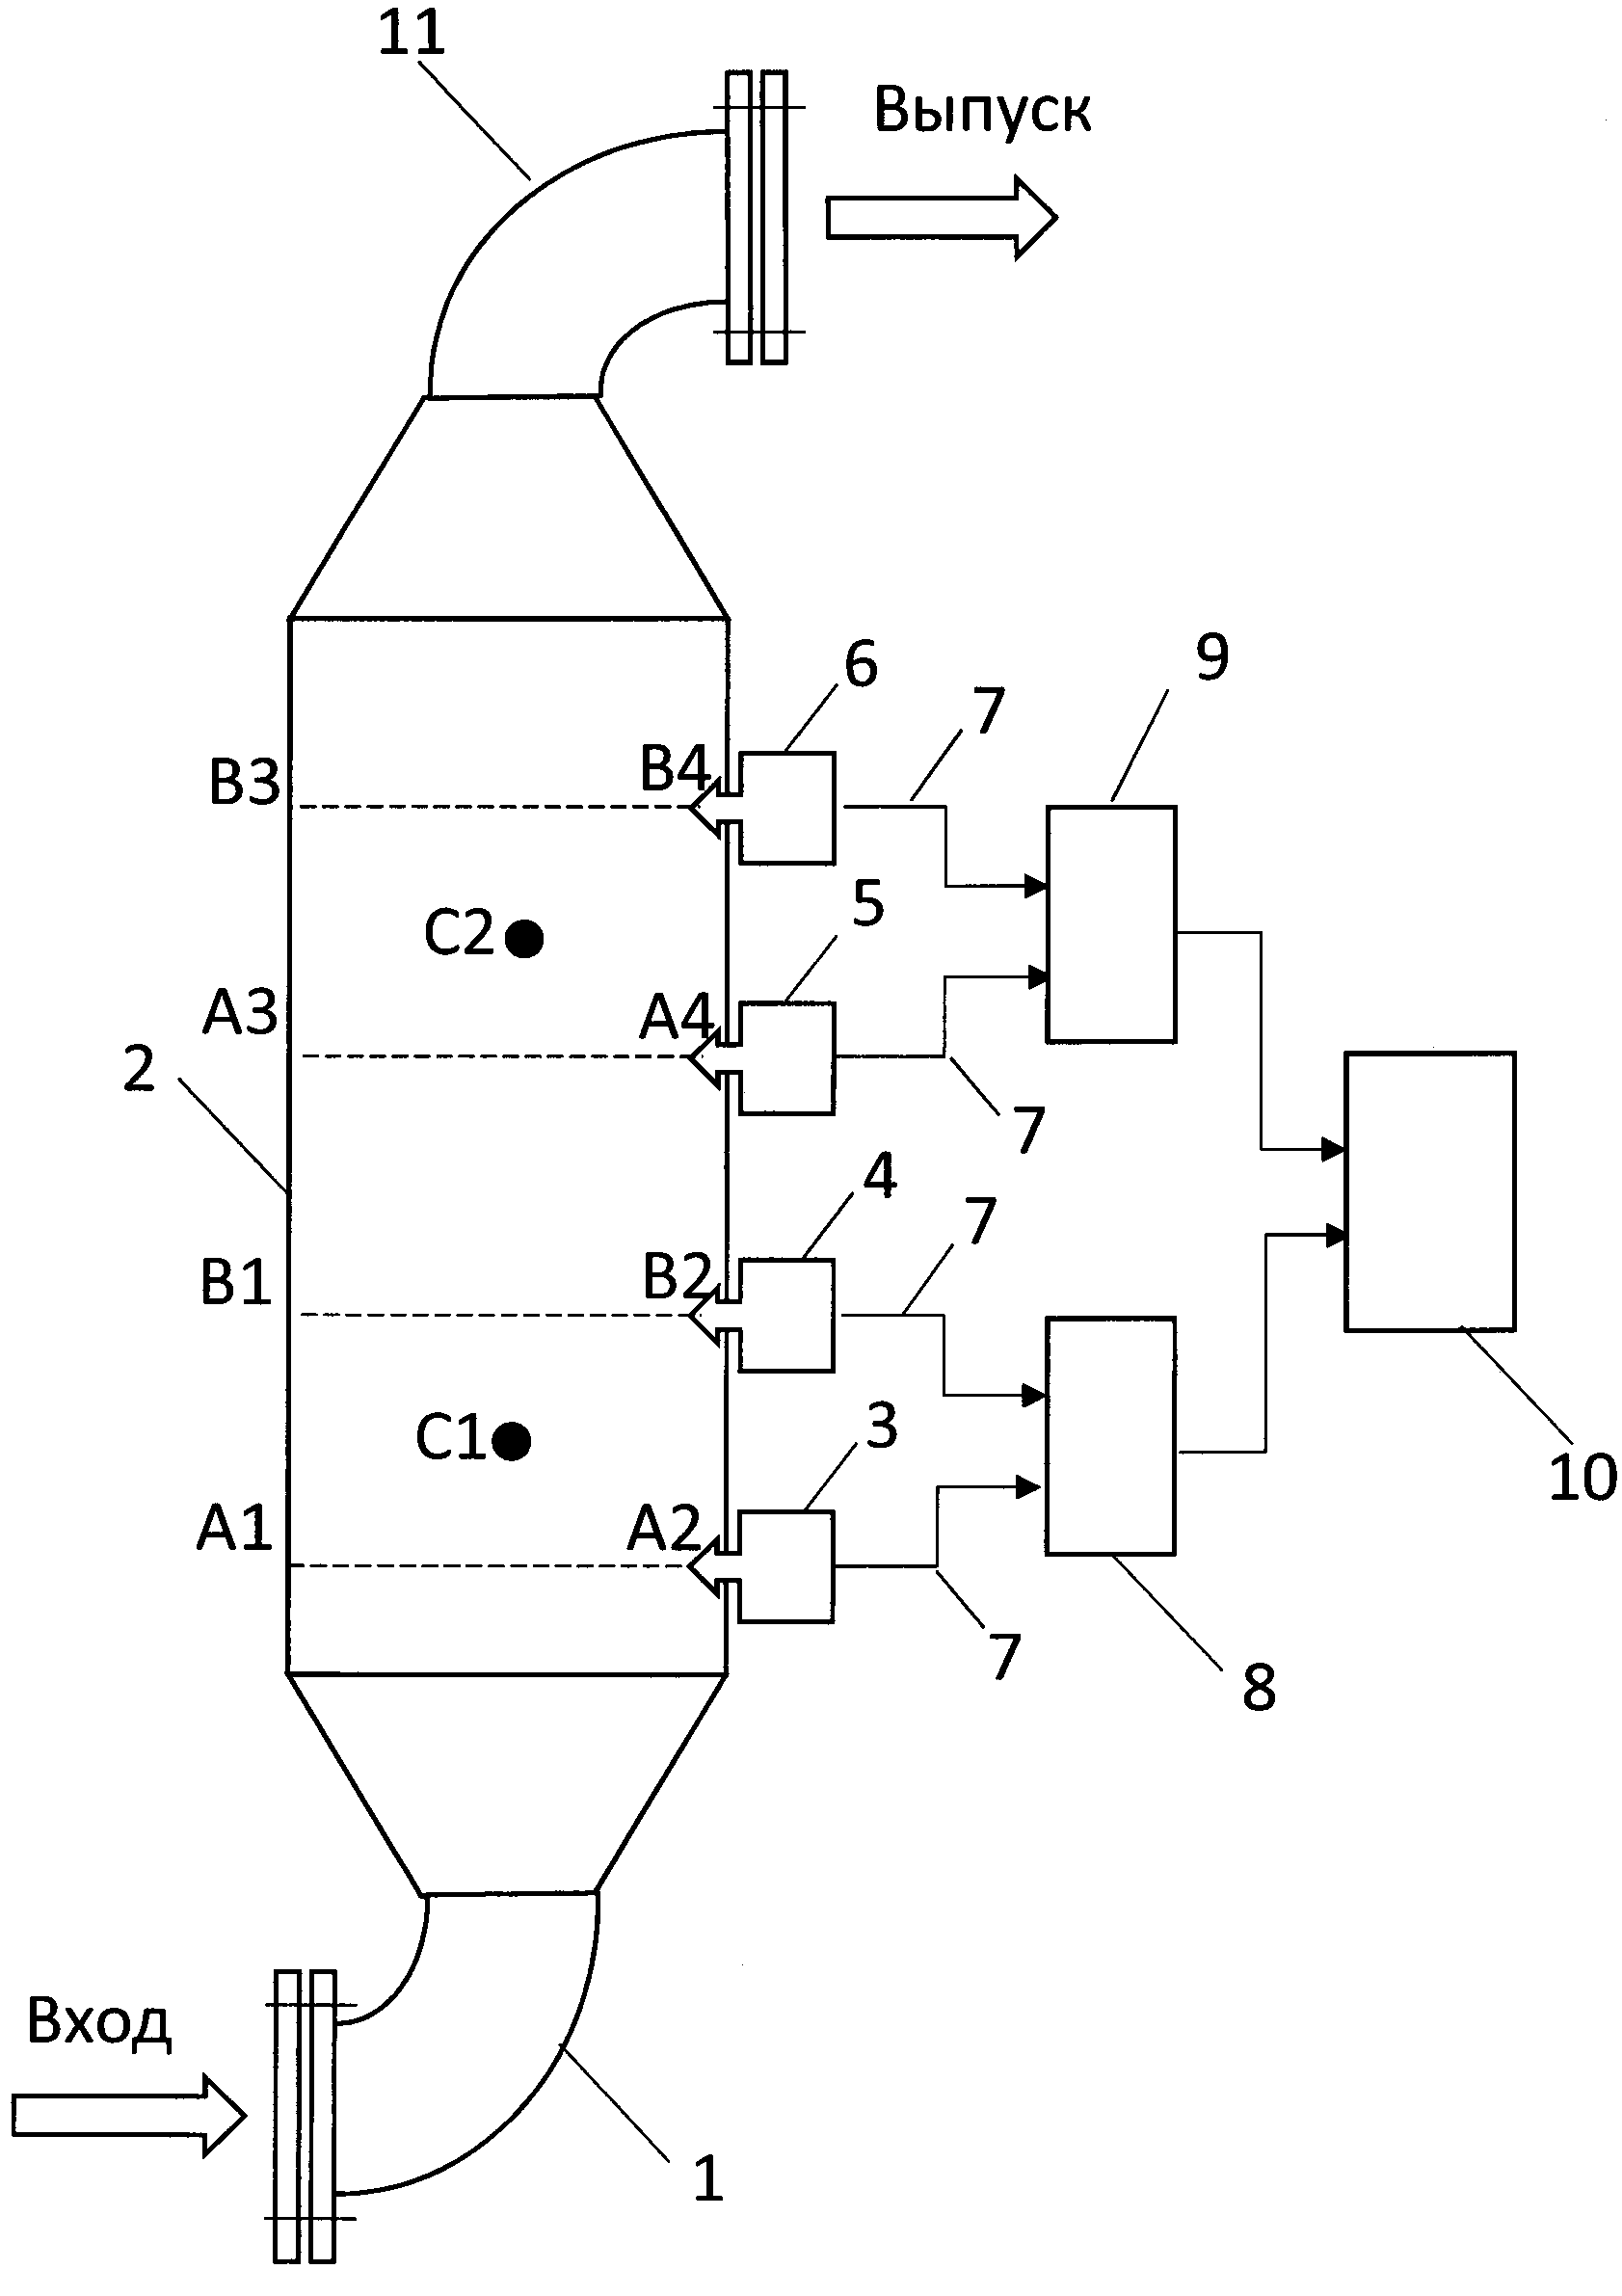
\includegraphics[width = 0.4\textwidth] {HydrostaticDensityMeter.png}
	\caption{Устройство для измерения плотности и расхода жидкости}
\end{figure}

\newpage
Данное устройство содержит впускной патрубок 1, напорный трубопровод 2, устройства 3, 4, 5 и 6 отбора давления, импульсные линии 7, датчики перепада давления 8 и 9, вычислительное устройство 10, выпускной патрубок 11. \par

Измерив при помощи датчиков давления 3 - 6 мы можем найти разность давления:
\begin{align}
	\Delta P_1 & = P_2 - P_1 \\
	\Delta P_2 & = P_4 - P_3
\end{align}
где $P_1$ и $P_2$ - величины давлений пульпы, измеренных на нижней и верхней границах 1-го участка; $\Delta P_1$ - величина перепада давления на первом участке. Аналогично для второго участка. \par

Теперь воспользовавшись выражением (9) можем найти значение плотности данной жидкости.

\begin{equation}
	\rho = \frac{\Delta P_1}{gh}
\end{equation}

Хочется также дополнить, что расстояние между двумя точками измерения давления определяется из пределов измерения плотности и давления: 

\begin{equation}
	\begin{cases}
		\Delta P_{max} = gh \rho_{max} \\
		\Delta P_{min} = gh \rho_{min}
	\end{cases}
\end{equation}

Данный прибор обладает высокой погрешностью - $\pm 1$\% диапазона шкалы. Такими плотномерами можно измерять плотность вязких, загрязненных, кристаллизующихся и агрессивных жедкостей, они пригодны как для открытых, так и для закрытых резервуаров. Их показания не зависят от скорости потока жидкости и ее поверхностного натяжения. \par

Из недостатков хочется отметить, что для высокой точности требуется большая высота столба, что делает прибор довольно громоздким.

\newpage

\subsection{Вибрационный плотномер}

На рисунке 3 представлена упрощенная схема вибрационного плотномера. Данный прибор относится к частотному типу вибрационных плотномеров, в которых измеряют функционально связанную с плотностью вещества частоту собственных колебаний резонатора.
\begin{figure}[h!]
	\centering
	\begin{tikzpicture}
		%\draw[gray, dashed] (0, 0) grid (15, 6);
		\draw (7, 3) node {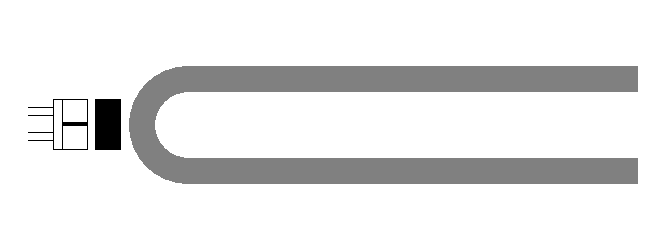
\includegraphics {VibratingDensityMeter.pdf}};
		\draw[thick, ->] (3.1, 5.1) -- (3.1, 3.45); \draw (3.1, 5.1) node[anchor = south] {Магнит};
		\draw (12.5, 3) node {Измерительная трубка};
		\draw[thick, ->] (2.7, 1.5) -- (2.7, 2.6); \draw (1.5, 1.5) node[anchor = north west] {Контроллер колебаний/измеритель колебаний};
	\end{tikzpicture}
	\caption{Упрощенная схема плотномера DE40/DE45}
\end{figure}

Здесь контроллер колебаний, переставляющий собой катушку индуктивности с переменным напряжением определенной частоты, изменение магнитного поля катушки заставляет магнит, то отталкиваться, то притягиваться, что вызывает колебания измерительно трубки с измеряемой жидкостью. \par

Период колебаний $T$ системы определяется следующим выражением:
\begin{equation}
	T = 2\pi \sqrt{\frac{\rho V_c + m_c}{K}}
\end{equation}
здесь $\rho$ - плотность содержимого трубки, $V_c$ - объем внутренней части трубки, $m_c$ - масса трубки, $K$ - коэффициент жёсткости трубки. \par

Теперь можем получить выражение для плотности: 
\begin{equation*}
	\rho = \frac{K}{4\pi^2 V_c}T^2 - \frac{m_c}{V_c} = AT^2 + B
\end{equation*}

Далее измерения можно упростить, введя $\rho_W$ - плотность воды, $\rho_A$ - плотность воздуха. Найдем их разность, полюзуясь выражением (15), получим:
\begin{equation*}
	\rho_A - \rho_W = A(T_A^2 - T_W^2)
\end{equation*}

Тогда можем найти коэффициент $A$:

\begin{equation*}
	A = \frac{\rho_A - \rho_W}{T_A^2 - T_W^2}
\end{equation*}
данную процедуру также называют калибровкой плотномера.

И поскольку плотность воздуха $\rho_A$ ялвяется табличной величиной, его можно использовать при измерении искомой плотности жидкости $\rho_S$.

\begin{equation*}
	A(T_A^2 - T_S^2) = \rho_A - \rho_S
\end{equation*}

В итоге получим искомое значение плотности жидкости:
\begin{equation}
	\rho_S = \rho_A - A(T_A^2 - T_S^2)
\end{equation}

Как видно из выражения (15) пределы измерения зависит от жесткости и объема трубки, а также от частоты колебаний контроллера. \par
Основным достоинством данных плотномеров является высокая точность, чувствительность и надежность. \par
Вместе с тем частотные плотномеры обладают и недостатками, к которым относятся ограниченность допускаемого расхода вещества определяемого площадью сечения канала, нелинейность шкалы. \par


\newpage

\subsection{Ультразвуковой плотномер}

Принцип работы ультрозвуковых плотномеров основан на распространении ультразвуковых колебаний (частота колебаний $ f > 20$ кГц) в исследуемой среде. По принципу работы УЗ-плотномеры разделяют на:
\begin{itemize}
	\item скоростное
	\item импедансные
	\item импедансно-скоростные
\end{itemize}

Ниже на рисунке представлен прибор для измерения плотности в экстремальных условиях. 
\begin{figure}[h!]
	\centering
	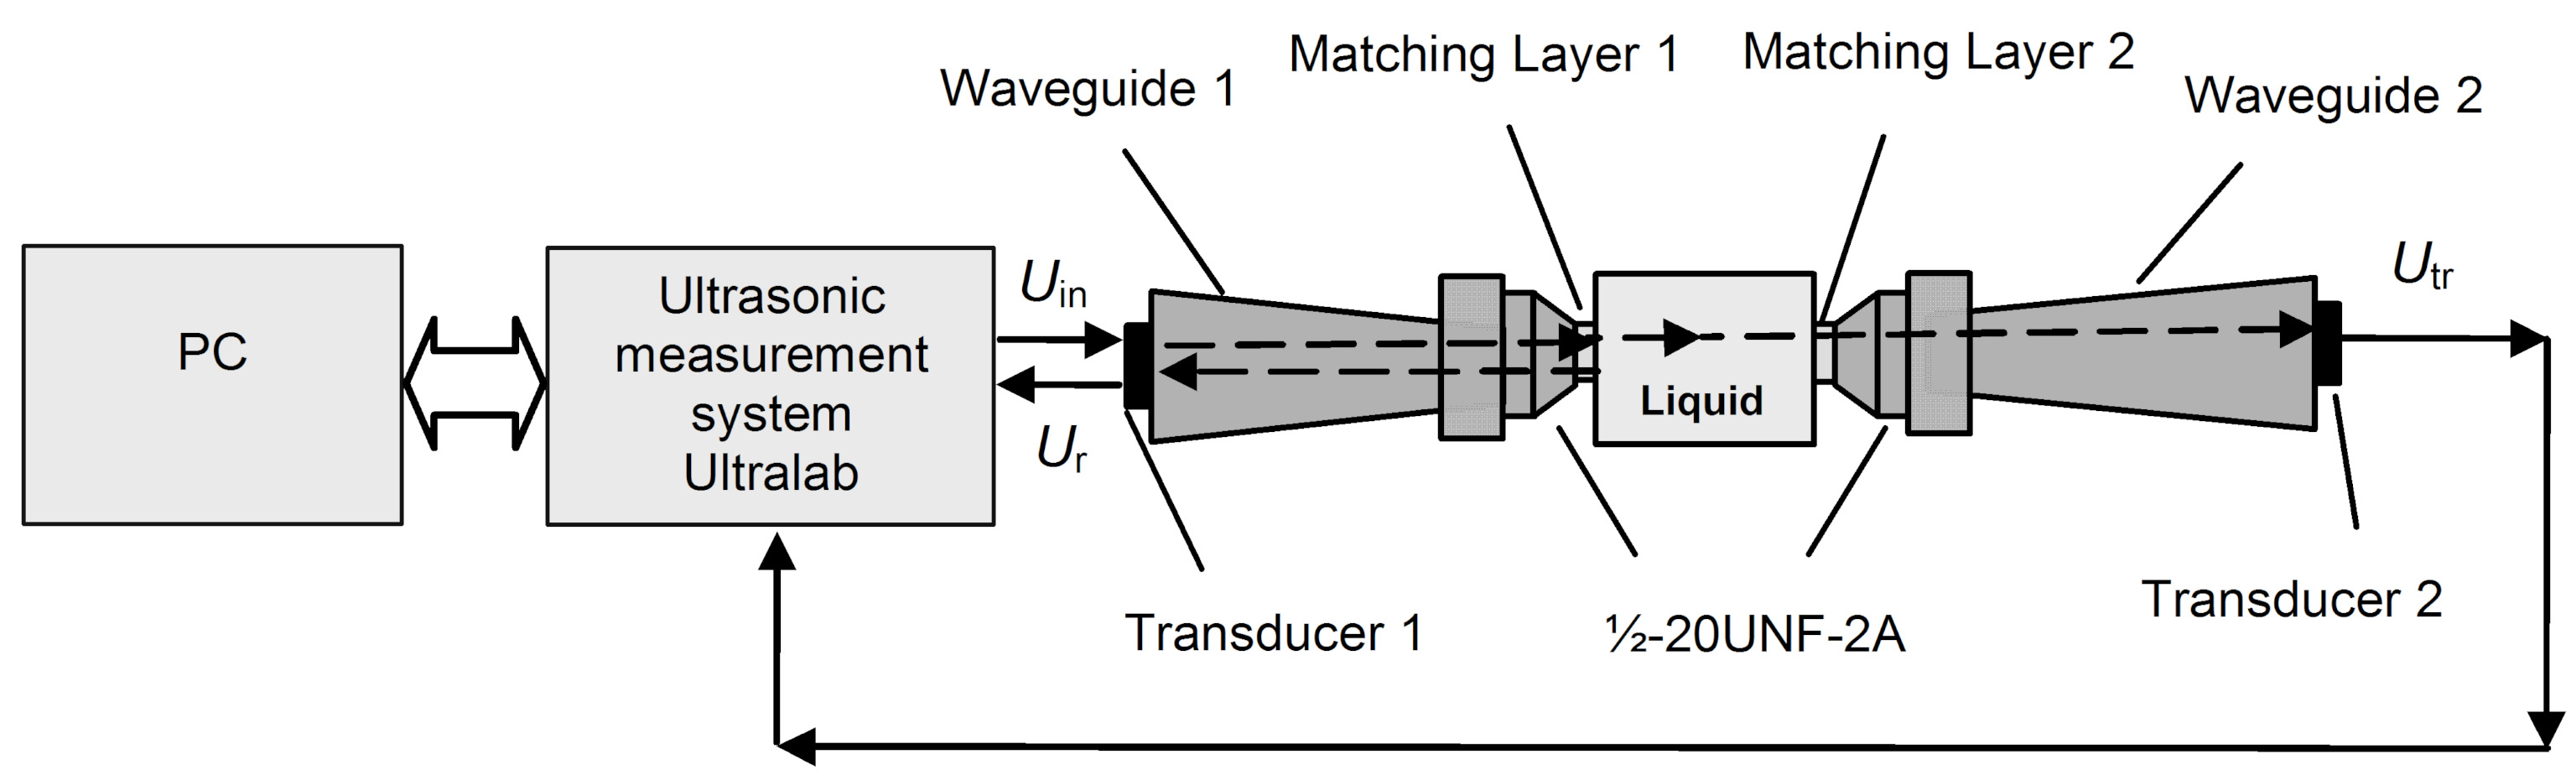
\includegraphics[width = 0.7\textwidth] {UltrasonicMeasuringSensor.png}
	\caption{Схема плотнометра с плавающим поплавком}
\end{figure}

Принцип работы данного прибора основан на определении акустического импеданса $Z_3$ жидкости и скорости распространения УЗ колебаний $c_3$ в данной среде. C плотносью эти две величины связвает следующее выражение: 
\begin{equation}
	Z_3 = \rho_3 c_3
\end{equation}

Система измерения плотности состоит из ультразвукового преобразователя (Ultrasonic Transducer 1), пьезоэлемента, который выполняет функции, как генератора колебаний, так и приемника; ультразвукого датчика (Ultrasonic Transducer 2); волноводов 1 и 2 (waveguides) с акустическими импедансами $Z_1$; двух смеживающий слоев (Matching Layer) с импедансами $Z_2$, соединяющих жидкость (Liquid) c импедансом $Z_3$ и волноводы. \par 

Ультразвуковой преобразователь 1 генерирует УЗ колебания, которые проходят через измеряемую жидкость и доходят до УЗ-приемника. Передаваемый импульс $U_{tr}$ используется для измерения скорости ультразвука $c_3$ измеряемой жидкости. Часть УЗ волны будет отражаться от границы раздела двух сред из-за несоответствия акуститеских импедансов $Z_2$ и $Z_3$ между волноводом и измеряемой жидкостью. Из принимаемого сигнала используется максимальное значение $U_r$ для определения плотности $\rho_3$. \par
Измерение плотности достигается измерением коэффициента отражения $R_3$ ультразвуковой волны от раздела жидкость/волновод. Данный коэффициент находится из отношения между амплитудами принимаемого и передаваемого сигнала.
\begin{equation}
	R_3 = \frac{U_{in}}{U_r}
\end{equation}

Коэффициент $R_3(\omega)$ зависит от частоты сигнала и может быть найден из следующего из следующего выражения: 

\begin{equation}
	R_3(\omega) = \frac{Z_{IN}(\omega) - Z_1}{Z_{IN}(\omega) + Z_1}
\end{equation}
где $Z_{IN}(\omega)$ входной акустический импеданс смеживающего слоя который определяется (при определенных условиях) следующим выражением : 

\begin{equation}
	Z_{IN} = \frac{Z^2_2}{Z_3}
\end{equation}
где $Z_2$ - акустический импеданс смеживающего слоя.

Подставляя (18) в (19) можем выразить импеданс жидкости $Z_3$.
\begin{equation}
	Z_3 = \frac{Z_2^2 (1 - R_3(\omega))}{Z_1 (1 + R_3(\omega)}
\end{equation}

Поскольку пьезоэлемент 1 не может одновременно излучать и измерять, амплитуду $U_{in}$ нельзя измерить, в противном случае нужны дополнительные датчики для ее измерения. Чтобы это нивелировать можно измерить коэффициент отражения $R_{3w}$ дистиллированной воды через амплитуду отраженного сигнала $U_{rw}$. И через отношение этих величин мы можем найти коэффициент отражения исследуемой жидкости.
\begin{equation}
	R_3(\omega) = \frac{U_r}{U_{rw}} R_{3w}(\omega)
\end{equation}

Подставляя полученные выражения (20), (21) в (16) можем найти плотность исследуемой жидкости.

\newpage
\section{Функциональная схема устройства}

Разберем функциональную схему ультразвукового плотномера.
\begin{figure}[h!]
	\begin{center}
	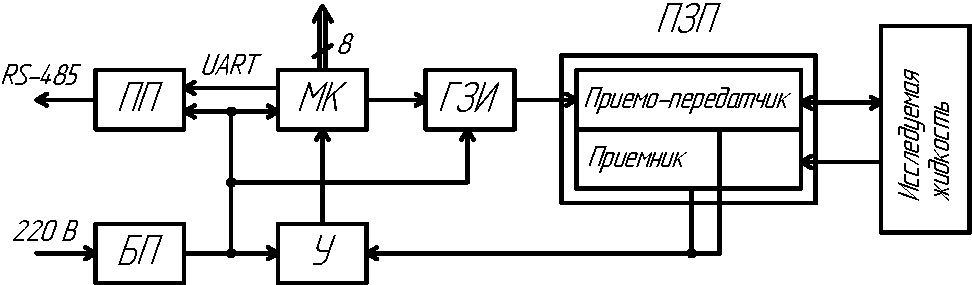
\includegraphics[width = 0.9\textwidth] {FuncScheme.pdf}
	\end{center}
	\caption{Функциональная схема: ПП - приемопередатчик, МК - микроконтроллер, ГЗИ - генератор зондирующих импульсов, ПЗП - пьезоэлектрический преобразователь, ПД - пиковый детектор, У - усилитель, БП - блок питания}
\end{figure}

Блок питания мощностью в 5 Ватт преобразует 220 вольт переменного напряжения в 5 вольт постоянного. Это питание подается на микроконтроллер, приемопередатчик, усилитель и генератор зондирующих импульсов. Как только приходит сигнал по RS-485 на микроконтроллер о том, что необходимо измерить плотность. Микроконтроллер подает сигнал на генератор зондирующих импульсов. Генератор формирует сигнал, в результате чего вызываются ультразвуковые колебания приемо-передатчика ПЗП. В результате отражения/прохождения колебаний в среде измерителя на приемник поступает сигнал, который фиксируется микроконтроллером и используется для измерения скорости звука измеряемой жидкости. На приемопередатчик же возвращается ультразвуковая волна, благодаря которой подсчитывается импеданс. Выходные сигналы поступаю с ПЗП на усилитель для анализа микроконтроллером с десяти-разрядного порта АЦП. 

\newpage
\section{Статический расчет и выбор элементов}
\subsection{Пьезоэлемент}
Рассчитаем пьезоэлемент, представленный на рисунке ниже. Частота собственных колебаний $f_0 = 1$ МГц. Материал ЦТС-19. \par 
\begin{figure}[h!]
	\begin{center}
	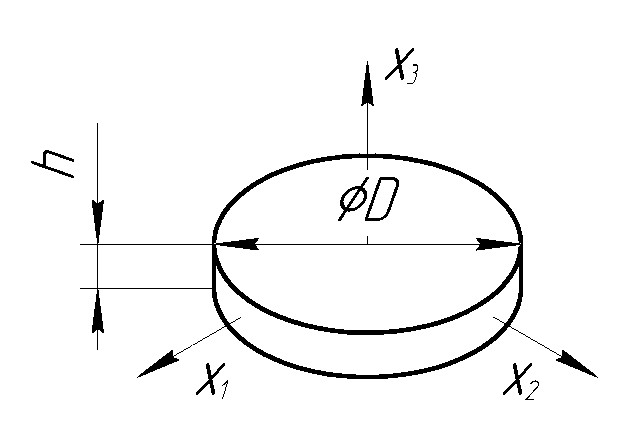
\includegraphics[width = 0.5\textwidth] {PiezoceramicScheme.pdf}
	\end{center}
	\caption{Пьезоэлектрик: h - ширина, D - диаметр}
\end{figure}
Для соблюдения резонансной частоты, необходимо, чтобы ширина пьезоэлемента была равна половине длинны волны. Из этого условия выведена формула для частоты собственных колебаний:
\begin{equation}
	f_0 = \frac{c}{2h}
\end{equation}
где $c$ - скорость звука в материале. По данной формуле можем найти ширину пьезоэлектрика:
\begin{equation}
	h = \frac{v_1}{2f_0} = \frac{3\cdot 10^3}{2\cdot10^6} = 0.0015 \text{ м} = 1.5\text{ мм}
\end{equation}

Теперь можем найти диаметр диска, для упрощения рассчетов, возьмем его на порядок больше толщины:
\begin{equation}
	D = 10h = 15 \text{ мм}
\end{equation}

Запишем выражения для обратного пьезоэфекта:
\begin{equation}
	u = d_{33} U_\text{ПЭП}
\end{equation}
где $u$ - деформация, м, $d_{33}$ - пьезомодуль.

Разложим подаваемое напряжение в ряд Фурье и оставим только первую гармонику. Она имеет вид: 
\begin{equation}
	U_\text{ПЭП} = U_m \sin{(\omega_0 t)}, \text{    } t \in [0, \tau]
\end{equation}
здесь $\omega_0 = 2 \pi f_0$ - круговая частота, $\tau = \displaystyle\frac{1}{2f_0}$ - длительность импульса, $U_m$ - амплитуда напряжения. Подставим выражение (26) в выражение (25).
\begin{equation}
	u = d_{33}U_m\sin{(\omega_0 t)}, \text{    } t \in [0, \tau] 
\end{equation}

Учитывая, что $v = \frac{du}{dt}$ - амплитуда колебаний скорости частиц, а генерируемая волна - синусоидальная бегущая. Запишем выражение для интенсивности ультразвука $I$.

\begin{equation}
	I = \frac{v^2 \rho c}{2} = \frac{d_{33} U_m \omega_0 \rho c}{2} \cos{(\omega_0 t)} = I_0 \cos{(\omega_0 t)}
\end{equation}

Акустический импуданс пьезокерамики ЦТС-19.

\begin{equation}
	Z_\text{0} = \rho c = 7.6 \cdot 3 \cdot 10^6 = 22.8 \cdot 10^6 \text{ Па}\cdot\text{с/м}
\end{equation}

Средний импеданс измеряемой жидкости.
\begin{equation}
	Z_\text{ж.ср} = 1.3 \cdot 10^6 \text{ Па}\cdot\text{с/м}
\end{equation}

Обычно пьезоэлектрический материал с высоким коэффициентом электромеханической связи имеет большое волновое сопротивление по сравнению с водой и воздухом. Поэтому, полоса пропускания частотной характеристики диска ниже. Неподходящее волновое сопротивление можно преодолеть, используя передний (согласующий) и задний (демпфер) слои между пьезоэлектрическим диском и жидкой средой. \par

На основании импедансов (29) и (30) выберем импеданс согласующего слоя, толщина которого $h_\text{согл.} = \lambda/4 = 0.75$ мм.

\begin{equation}
	Z_\text{согл.} = \frac{Z_\text{пэ} + Z_\text{ж.ср}}{2} = 12 \cdot 10^6 \text{ Па}\cdot\text{с/м}
\end{equation}
Таким импедансом обладает керамика $SiO_2$, чей импеданс равен $Z_{2} = 5.8 * 2.65 \cdot 10^6 = 15 \cdot 10^6 \text{ Па}\cdot\text{с/м}$

В качестве демпфера вьзмем эпоксидную смолу, смешанную с наполнителем из мелкодисперсного порошка вольфрама. Толщина демпфера равна $6$ мм. В итоге получим систему слоев для движения ультразвуковой волны (рисунок ниже).
\begin{figure}[h!]
	\centering
	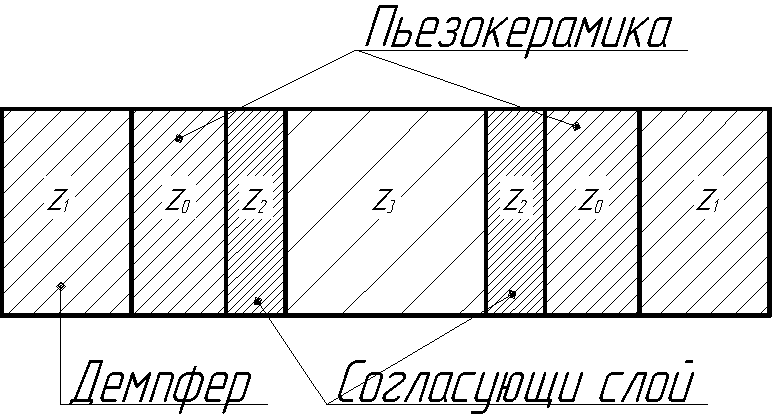
\includegraphics[width = 0.45\textwidth] {DensityMeterScheme.pdf}
	\caption{Cхема слоев ультразвукового плотномера}
\end{figure}

\newpage
\subsection{Усилитель напряжения}
Усилитель включен в нашу цепь с целью поднять напряжение, получаемое с пьезоэлемента, до уровня логической единицы микроконтроллера, то есть до уровня 2,6—5 В. Для этого нам необходимо знать параметры электрического сигнала, возбуждаемые в пьезоэлементе ультразвуковой волной. \par
Пранализируем, насколько уменьшится амплитуда акустического давления когда она пройдет через второй пьезоэлемент. Коэффициент затухания в воде при 1 МГц $\alpha \approx 0.5$.

\begin{equation}
	I_1 = I_0 e^{-\alpha L} = \frac{d_{33} U_m \omega_0 \rho c}{2} e^{-2\alpha L}
\end{equation}
здесь $L = 40$ мм - длинна полости для жидкости. Амплитуда интенсивоности изменится в $e^{-2\alpha L} \approx 0.67$ раза. Напряжение, подаваемое на первый пьезоэлемент примем равным $Um = 5$ В.  В итоге интенсивонсть будет равна.
\begin{equation}
	I_1 = \frac{3 \cdot 7.6 \cdot 6.28 \cdot 350 \cdot 5}{2} \cdot 0.67 = 8354 \text{ Вт/м}
\end{equation}

Оценим вернувуюся на первый преобразователь отраженную волну.
\begin{equation}
	I_2 = I_0R_{32} e^{-4\alpha L} = I_1 R_{32} e^{-2\alpha L}
\end{equation}

Амплитуда интенсивности зменитьв следующим образом.
\begin{equation}
	R_{32} e^{-4\alpha L} = \left( \frac{z_3 - z_2}{z_3 + z_2} \right)^2 \cdot e^{-4\alpha L} = 0.71 \cdot 0.45 = 0.32
\end{equation}
Как можно заметить амплитуда интенсивности упадет в 3 раза по сравнению с $I_0$. Таким образом, необходимо усилить напряжение в 2.5 раза.

В качестве усилителя будем использовать неинвертирующий усилитель на операционном усилителе, схема которого представлена на рисунке 7. 

\begin{figure}[h!]
	\begin{center}
	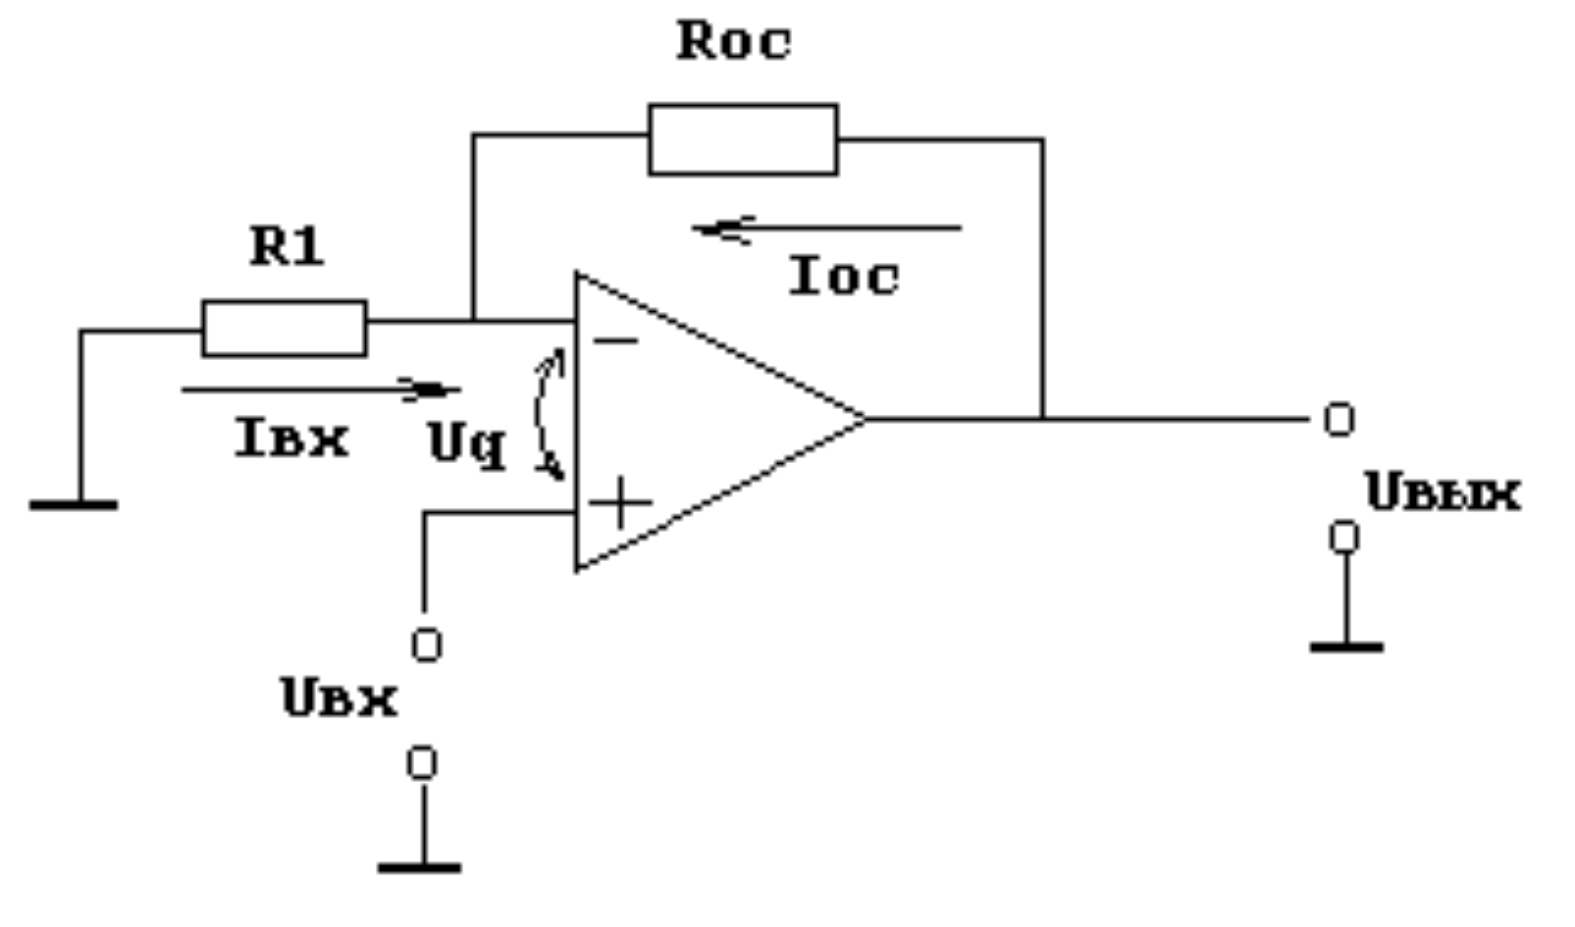
\includegraphics[width = 0.5\textwidth] {OY.png}
	\end{center}
	\caption{Усилитель напряжения}
\end{figure}

Коэффициент усиления данной схемы равен:
\begin{equation}
\frac{U_\text{вых}}{U_\text{вх}} = \frac{R_{oc} + R_1}{R_1} = 2.5
\end{equation}
Примем $R_1 = 1$ кОм, тогда не трудно найти $R_\text{ОС} = 1.5$ кОм.

Операционный усилитель представлен на микросхеме OPA341 и имеет следующие параметры.
\begin{itemize}
	\item Напряжение питания 5В
	\item Ток питания - 0.2 мА
	\item Потребляемая мощность - 1мВт
\end{itemize}
\subsection{Генератор зондирующих импульсов}
Для создания ультразвуковой волны на пьезоэлементе на него следует подать сигнал, который как можно быстрее увеличивается до своего максимального значения, а затем, как можно быстрее, угасает.\par
 Поскольку в нашем устройстве микроконтроллер проводит замер времени, который должен начинаться одновременно с созданием ультразвуковой волны, то генератор должен работать в ждущем режиме, в ждущем режиме и управляться импульсом, подаваемым с микроконтроллера. \par 
Схема генератора зондирующих импульсов представлена на рисунке ниже.

\begin{figure}[h!]
	\begin{center}
	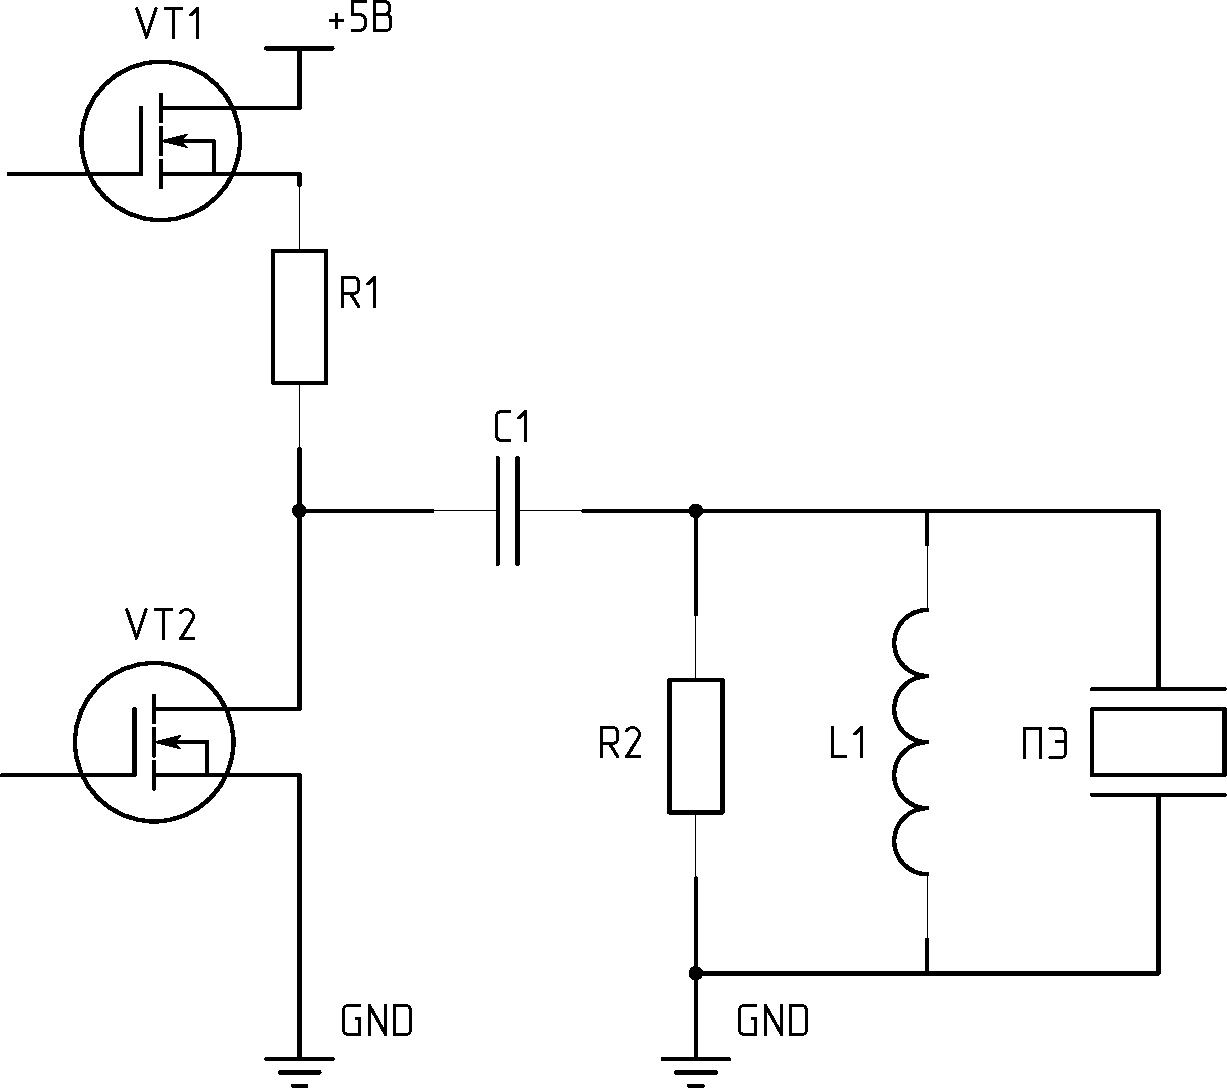
\includegraphics[width = 0.4\textwidth] {Generator.pdf}
	\end{center}
	\caption{Генератор зондирующих импульсов}
\end{figure} 


\subsection{Выбор приемопередатчика}
В качестве приемопередатчика выберем схему ADM1485JNZ фирмы Analog Devices, который будет подсоединяться к микроконтроллеру по протоколу UART.

\begin{itemize}
	\item Напряжение питания 5 В
	\item Ток питания - 1.35 мА
	\item Потребляемая мощность - 6.75 мВт
\end{itemize}
\subsection{Выбор микроконтроллера}
Для обработки сигналов с датчиков был выбран микроконтроллер ATtiny8303 фирмы Atmel. Микроконтроллер имеет встроенный АЦП, необходимый для обработки сигнала с усилителя, а так же поддерживает UART, необходимый для работы с приемопередатчиком RS-485.
\begin{itemize}
\item Напряжение питания - 5 В
\item Ток питания - 10 мА
\item Потребляемая мощность - 50 мВт
\end{itemize}
\subsection{Выбор блока питанияFR}
Для питания логических схем и генератора зондирующих импульсов необходимо получить напряжение напряжение 5В. Исходя из суммы полученных выше мощностей подходит блок питания AC Adapter pro-power со следующими характеристиками:
\begin{itemize}
\item Выходное напряжение - 5 В
\item Минимальный ток - 0.01 А
\item Выходная мощность - 5 Вт
\end{itemize}


\newpage
\section{Разработка принципиальной схемы устройства}
Произведём разработку принципиальной электрической схемы устройства, приняв за основу функциональную схему. Через разъем X1 подется преобразованное питание +5 вольт. \par
Через разъем X2 осуществляется прием и передача через интерфейс RS-485. Данный интерфейс переводится логическим устройством в интерфейс UART, понятный микроконтроллеру. \par
Порты X3 и X4 служат для снятия/подачи сигнала на пьезоэлектрический преобразователь. 

\newpage
{\StructSection{Заключение}
\addcontentsline{toc}{section}{Заключение}}

В ходе выполнения курсового проекта был показан процесс разработки преобразователя информации по заданному техническому заданию. \par
Результатом работы является спроектированное устройство для из-
мерения плотности жидкости. Используется ультразвуковой импедансно-временной метод. В качестве излучателей/приемников исплользуются пьезоэлементы. \par
Спроектированне устройсто обладает малыми габаритами, высоким быстродействием и точностью. Данный прибор приспособен для лабораторных условий. Для промышленных целей он не годится. 

\newpage
%
% ----------------------------------------------------------------------
% Refferences
\renewcommand\refname{Список использованных источников} % Невероятный костыль
\ESKDsectAlign{section}{Center}

\begin{thebibliography}{}
	\bibitem{Stewart} Stewart Sherrit, Binu K. Mukherjee. Characterization of Piezoelectric Materials for Transducers
	\bibitem{Barhatov} Бархатов В.А. Электромеханическая модель пьезопреобразователя.
	\bibitem{Sharapov} Шарапов В. М., Мусиенко М. П., Шарапова Е. В. Ш25 Пьезоэлектрические датчики / Под ред. В.М. Шарапова. - Москва: Техносфера, 2006. - 632 с.
	\bibitem{Kivilis} Кивилис С. С. Плотномеры.-М.:Энергия, 1980.-с., ил.
	\bibitem{Rymantas} Rymantas Kazys, Reimondas Sliteris, Regina Rekuviene, Egidijus Zukauskas and Liudas Mazeika. Ultrasonic Technique for Density Measurement of Liquids in Extreme Conditions

    \bibitem{litlink2}  Блинников А.А, Бойков В.И., Быстров С.В., Николаев Н.А., Нуйя О. С. Правила оформления пояснительной записки и конструкторской документации.–СПб: Университет ИТМО, 2014.–55 с.
\end{thebibliography}

\ESKDappendix{}{}
\begin{figure} [h!]
	\centering
	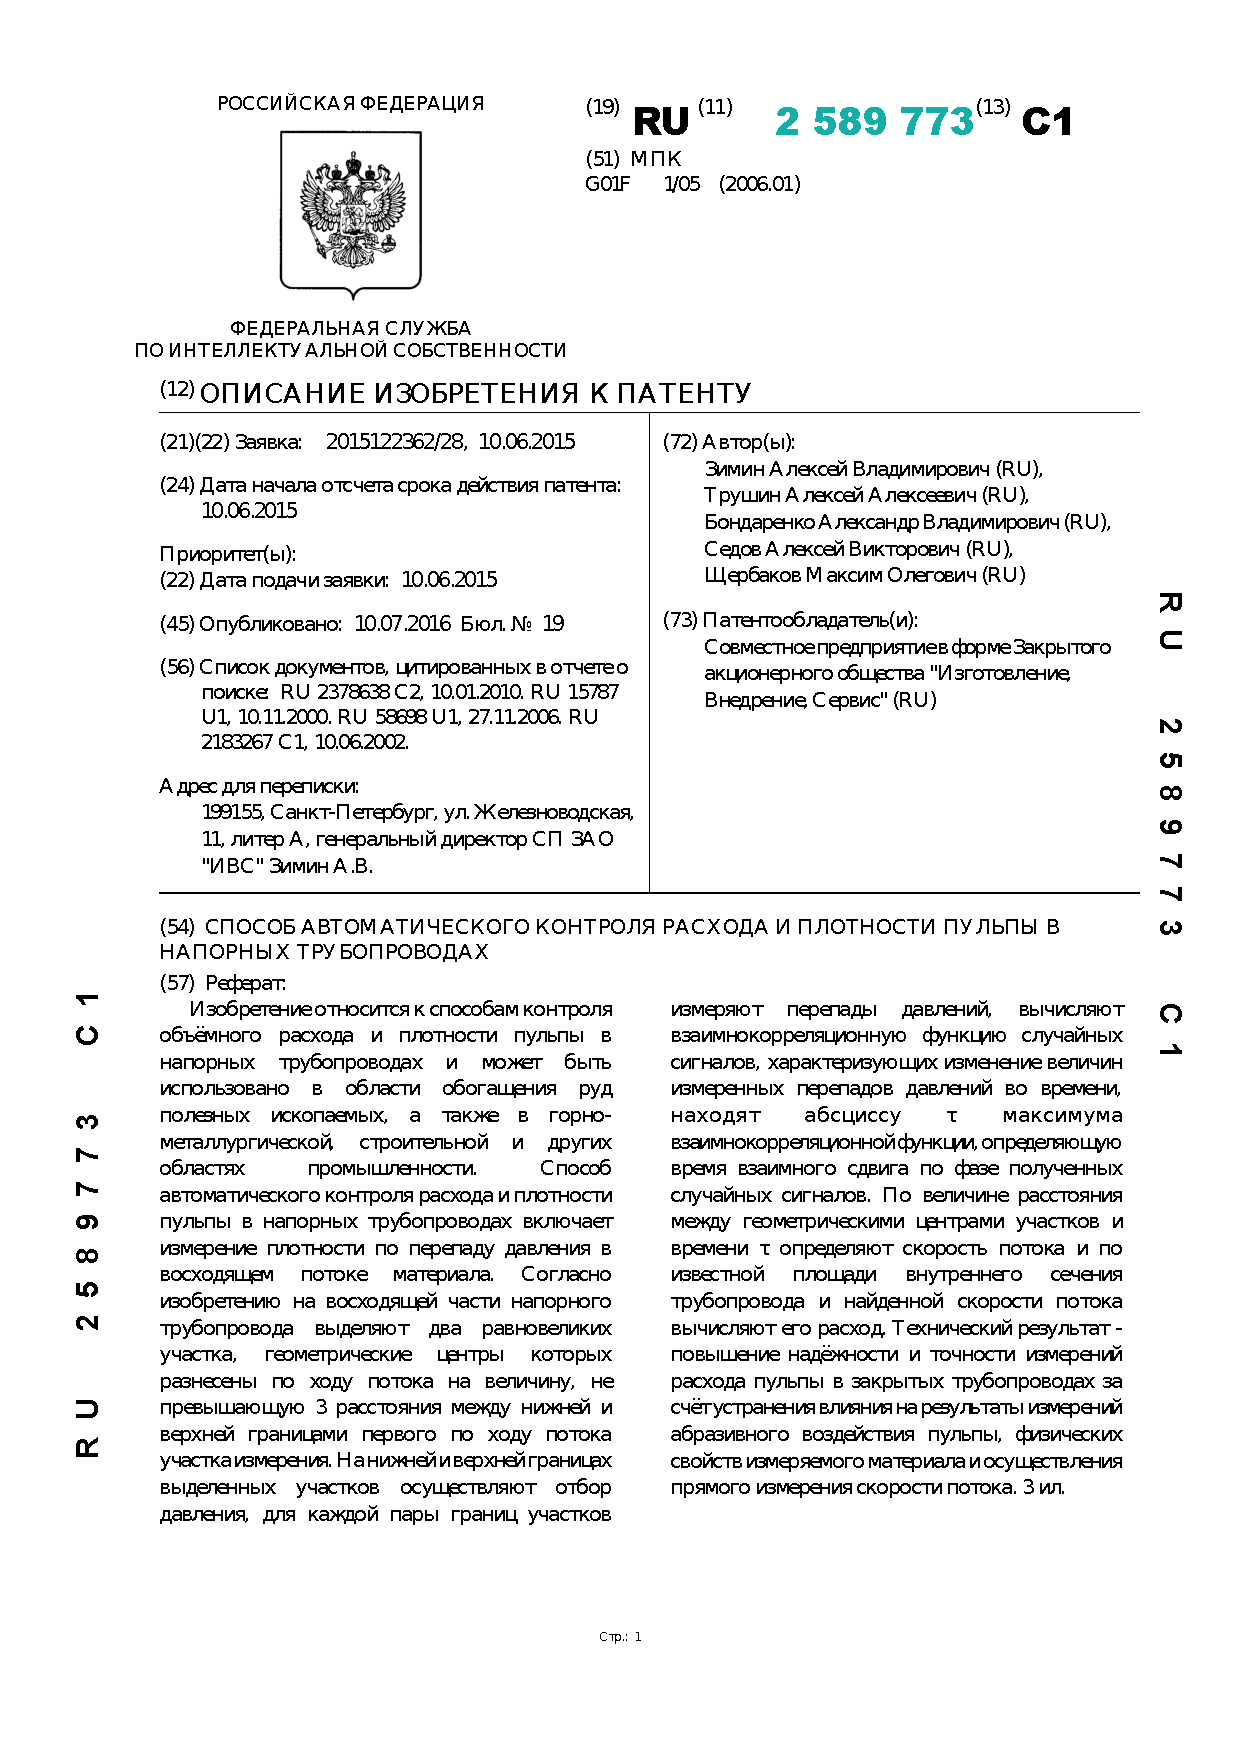
\includegraphics[width = 0.8\textwidth]{patent1-1.pdf}
\end{figure}
\begin{figure} [h!]
	\centering
	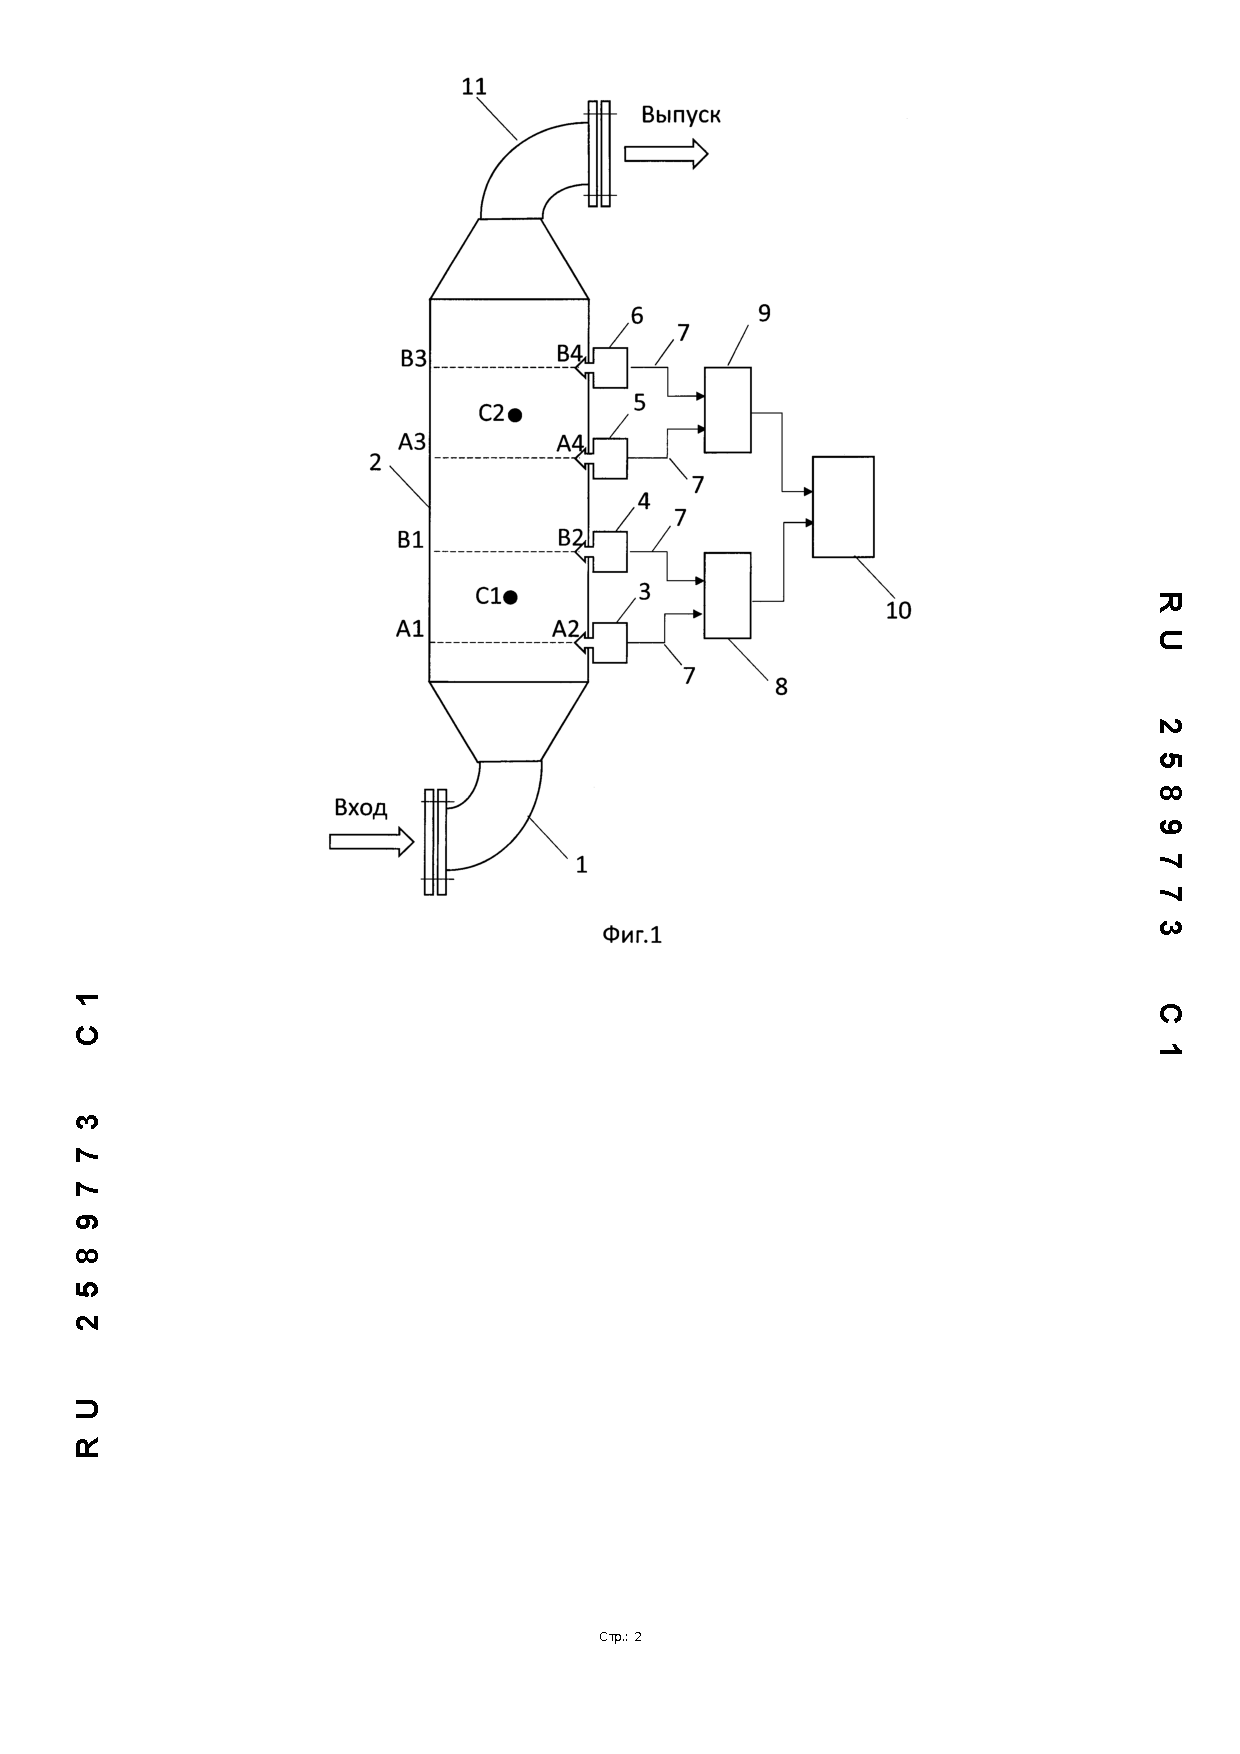
\includegraphics[width = 0.7\textwidth]{patent1-2.pdf}
\end{figure}
\ESKDappendix{}{}
\begin{figure} [h!]
	\centering
	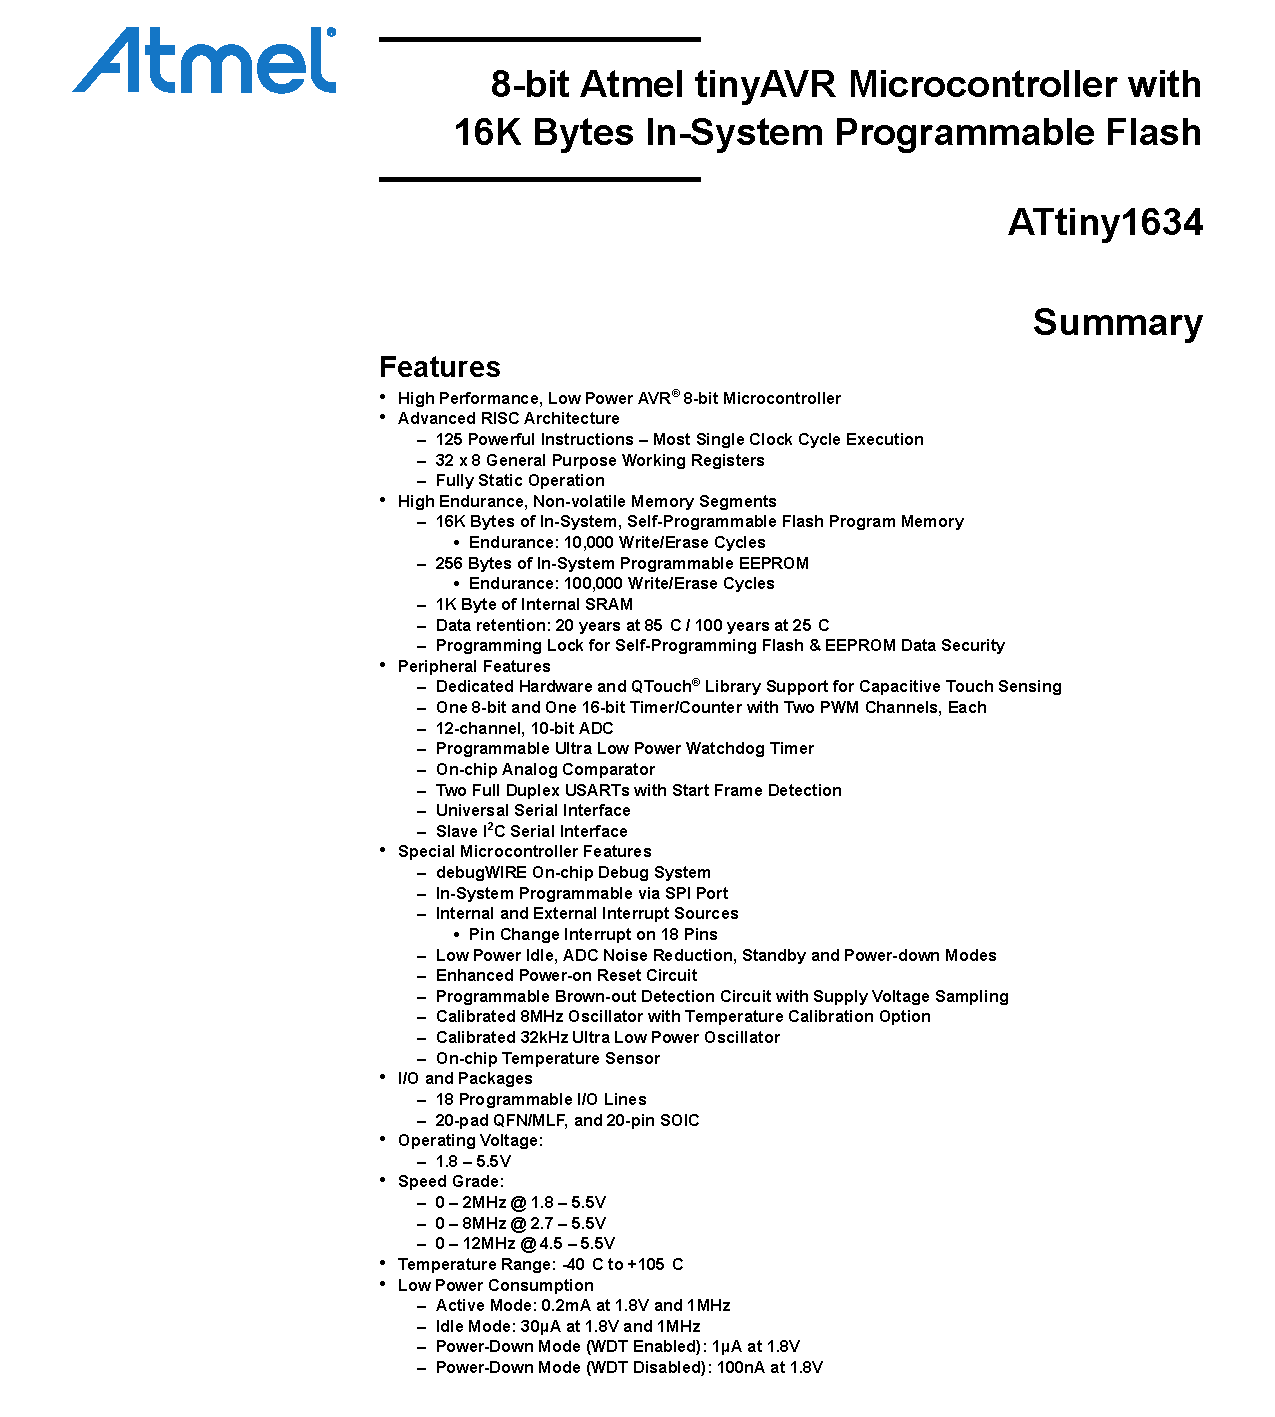
\includegraphics[width = \textwidth]{contoller-1.pdf}
\end{figure}
\begin{figure} [h!]
	\centering
	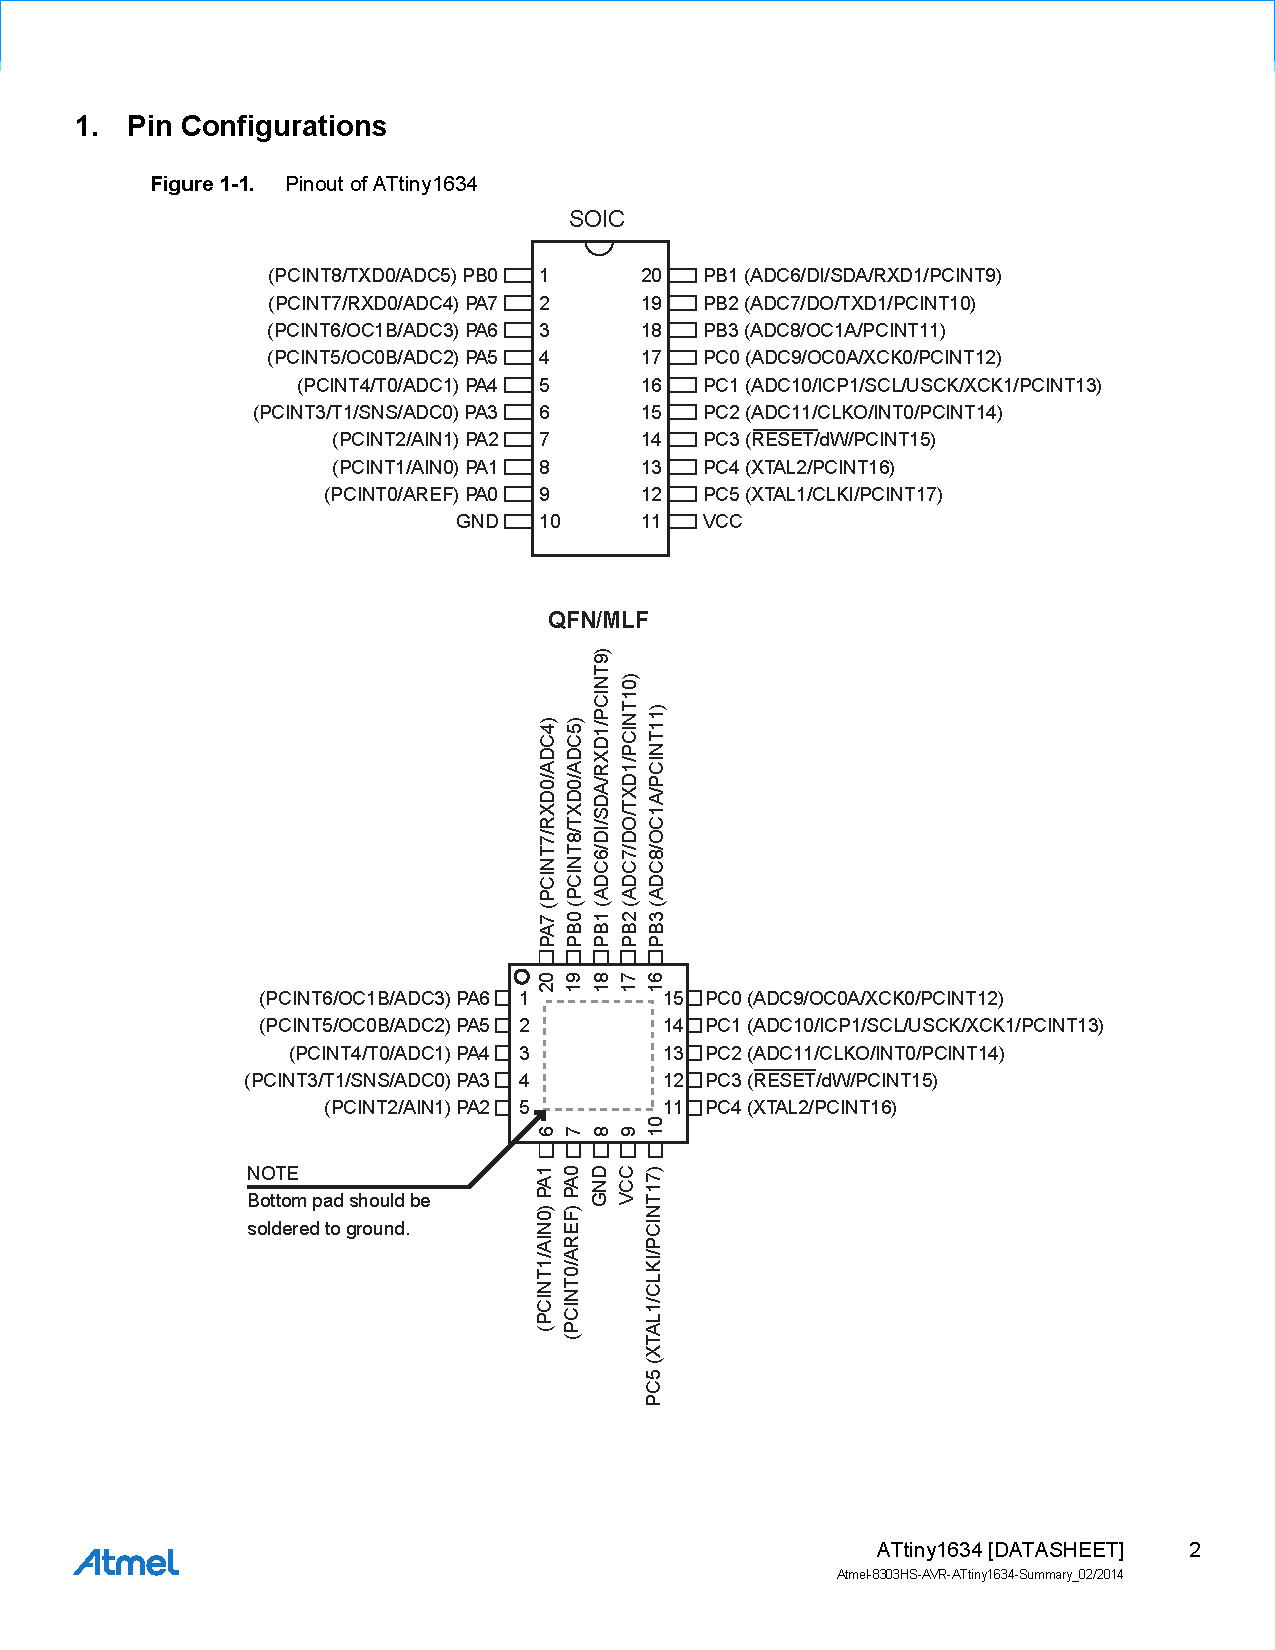
\includegraphics[width = \textwidth]{contoller-2.pdf}
\end{figure}

\ESKDappendix{}{}
\begin{figure} [h!]
	\centering
	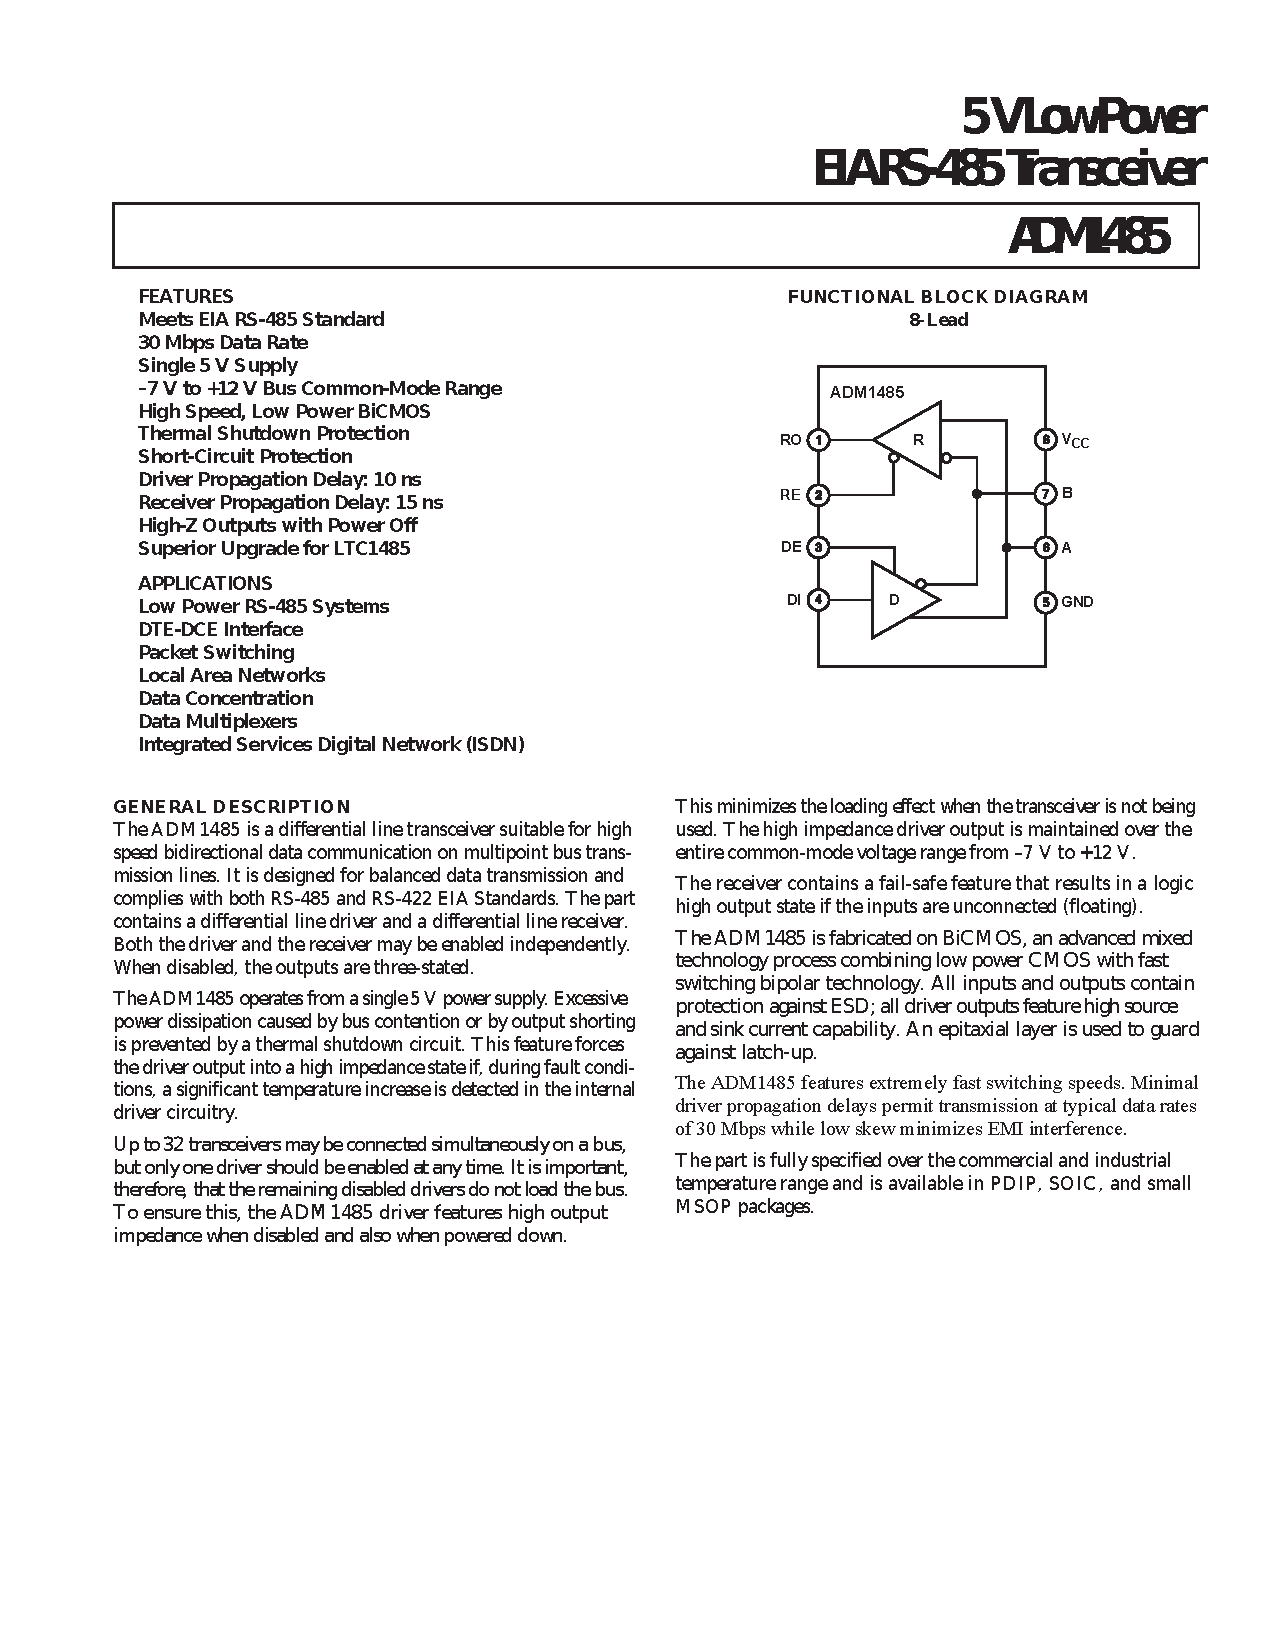
\includegraphics[width = 0.95\textwidth]{ADM1485-1.pdf}
\end{figure}

\ESKDappendix{}{}
\begin{figure} [h!]
	\centering
	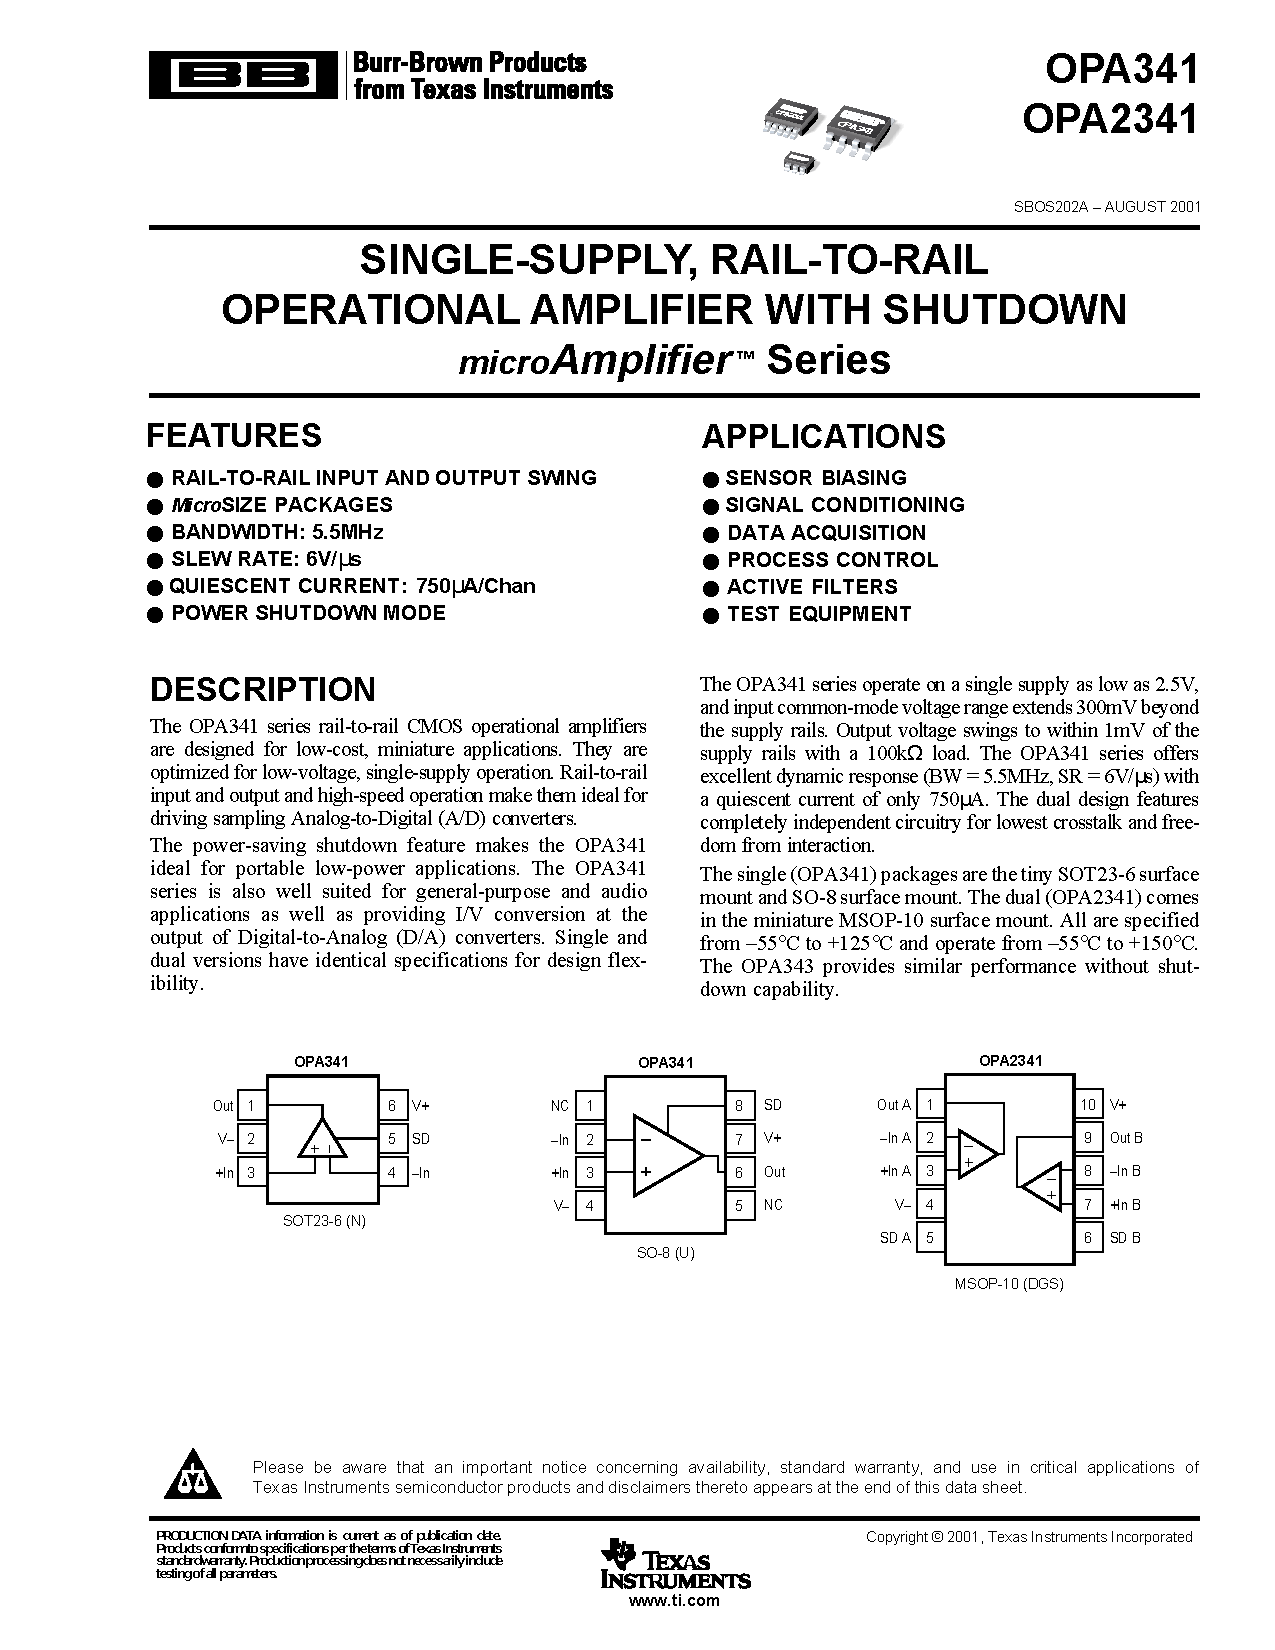
\includegraphics[width = 0.9\textwidth]{opa341-1.pdf}
\end{figure}
\begin{figure} [h!]
	\centering
	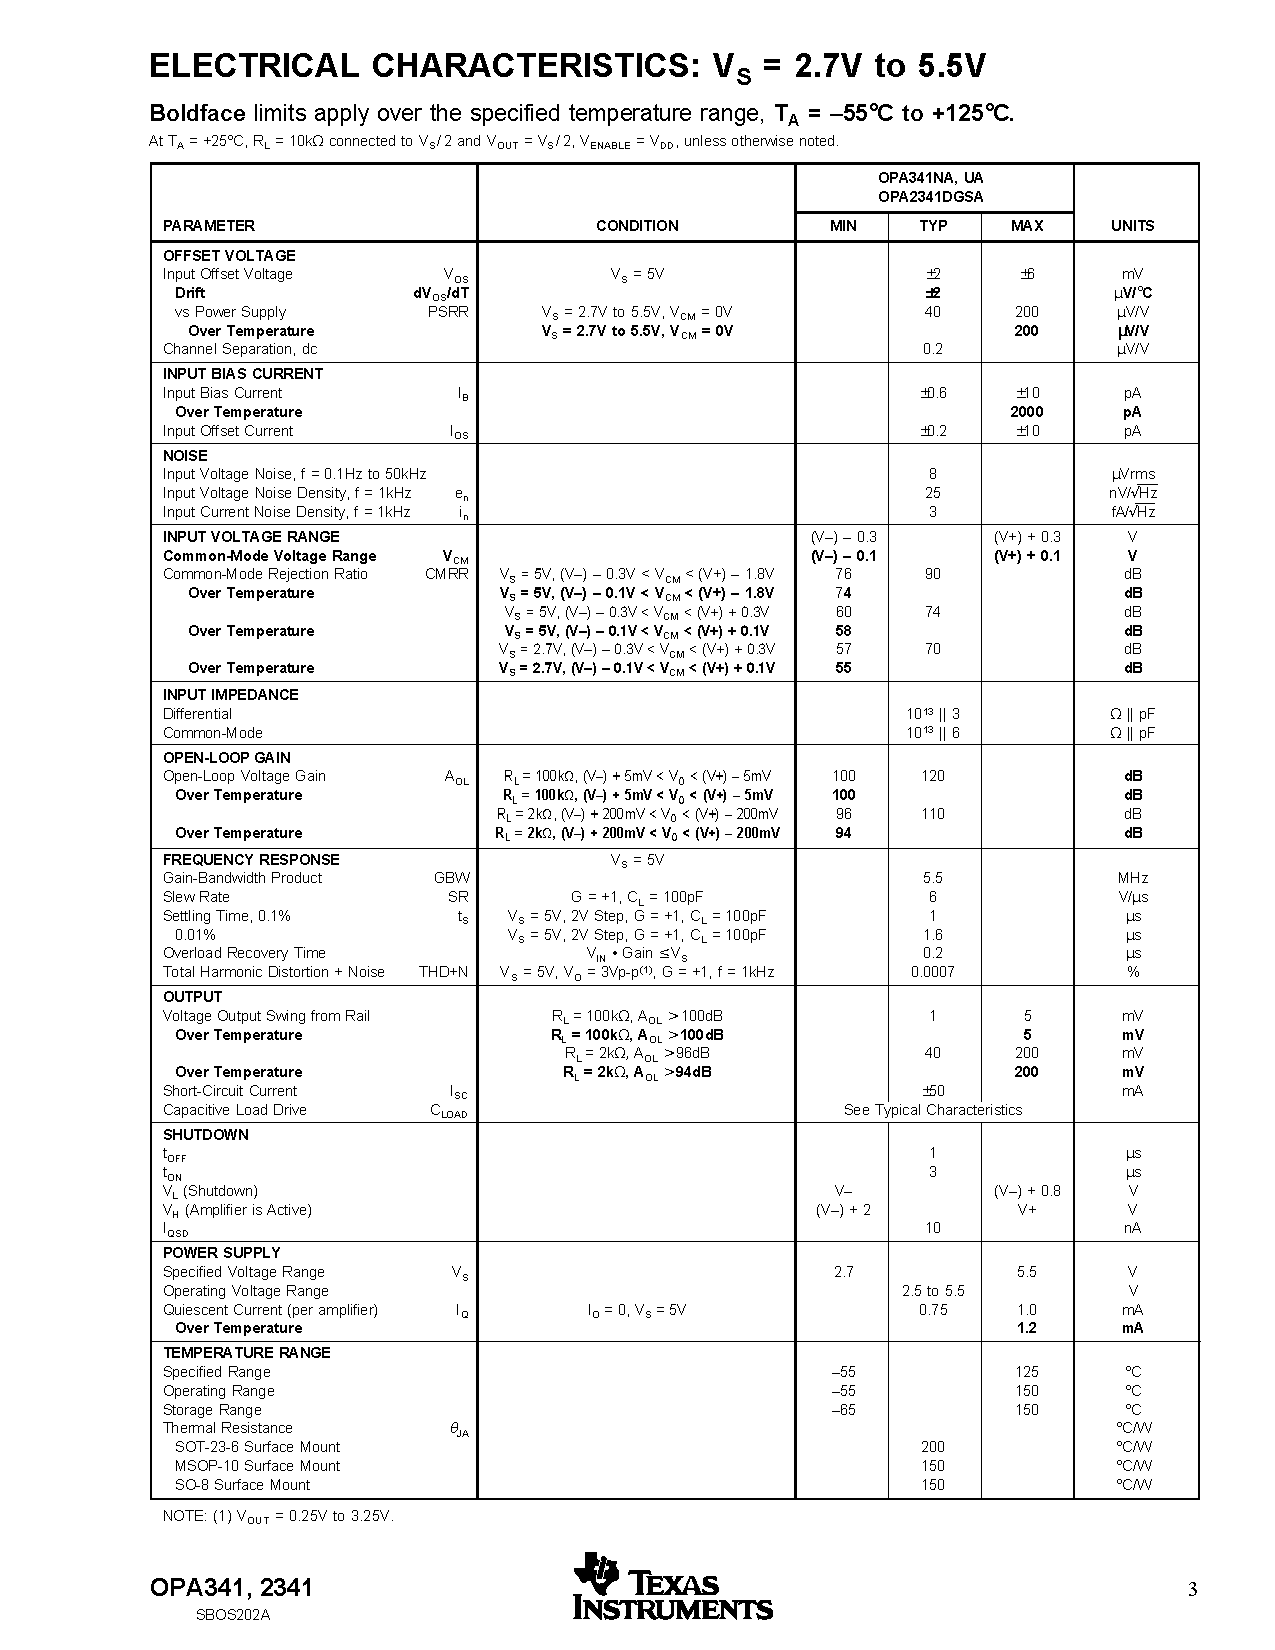
\includegraphics[width = 0.9\textwidth]{opa341-2.pdf}
\end{figure}

\ESKDappendix{}{}
\begin{figure} [h!]
	\centering
	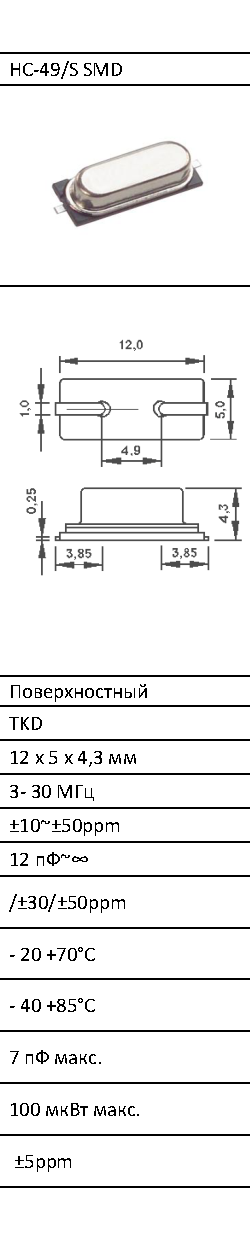
\includegraphics[width = 0.2\textwidth]{resonator.pdf}
\end{figure}

\end{document}
